\documentclass[12pt, twoside]{report}

\usepackage[utf8]{inputenc}
\usepackage[english]{babel}
\usepackage[a4paper,width=150mm,top=25mm,bottom=25mm,bindingoffset=6mm]{geometry}
\usepackage{caption}
\usepackage{subcaption}
\usepackage{color}
\usepackage{tikz}
\usepackage{amsmath}
\usepackage{amsfonts}
\usepackage[noend]{algpseudocode}

\usepackage{lipsum} 

\usepackage{tabularx}
\renewcommand{\arraystretch}{1.2}

\usepackage{mathtools}
\DeclarePairedDelimiter\ceil{\lceil}{\rceil}
\DeclarePairedDelimiter\floor{\lfloor}{\rfloor}

\usepackage{graphicx}
\graphicspath{ {images/} }

\usepackage{fancyhdr}
\pagestyle{fancy}
\fancyhead{}
\fancyhead[RO,LE]{Thesis Title}
\fancyfoot{}
\fancyfoot[LE,RO]{\thepage}
\fancyfoot[LO,CE]{Chapter \thechapter}
\fancyfoot[CO,RE]{Author Name}

\usepackage[backend=bibtex]{biblatex}  
\addbibresource{references.bib}

\newcommand{\note}[1]{\textcolor{red}{[#1]}}
\newcommand{\eqtab}{\;\;\;\;\;\;}

\title{Master Thesis}
\author{Maxime Schoemans}
\date{2019 - 2020}

\begin{document}

% Logos
\newcommand{\ulb}{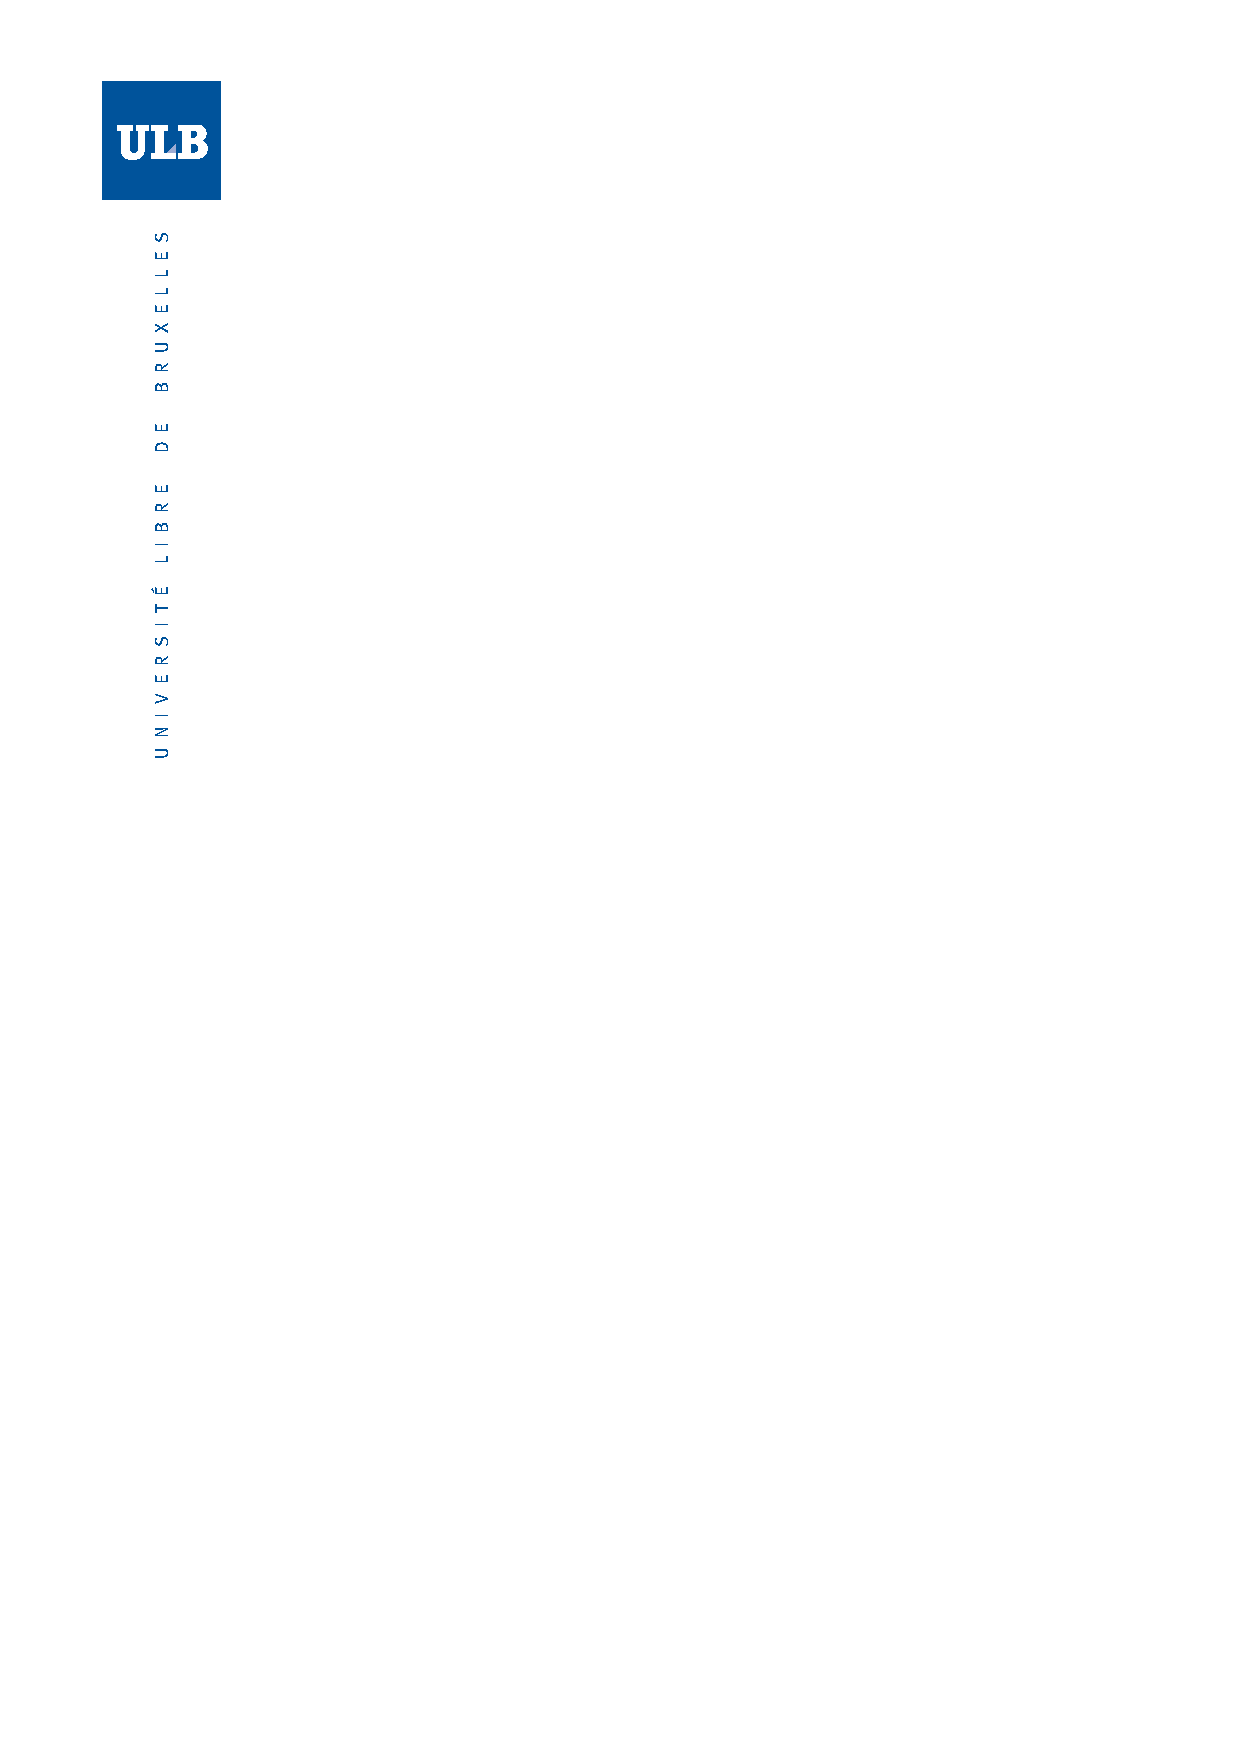
\includegraphics[scale=1.1]{logo_ULB2.pdf}}
\newcommand{\polytech}{
\includegraphics[scale=0.35]{logo_polytech_FR.pdf}}

% Polices
\definecolor{ULBblue}{rgb}{0,0.2196,0.5765}
\newcommand{\fontTitle}{\sffamily \Huge\selectfont \color{ULBblue}}
\newcommand{\fontSubtitle}{\sffamily \LARGE \selectfont \color{ULBblue}}
\newcommand{\fontText}{\sffamily \selectfont}
\newcommand{\fontColor}{\sffamily \selectfont \color{ULBblue}}

% Titre
\newcommand{\titleA}{\fontTitle{Première ligne de titre du mémoire}} % Titre identique au titre remis au secrétariat
\newcommand{\titleB}{\fontTitle{Deuxième ligne de titre du mémoire}} % (dans la langue de rédaction a priori)
% Sous-titre
\newcommand{\subtitle}{\fontSubtitle{Ligne du sous-titre du mémoire}}
% Titre du diplôme
\newcommand{\diplomaA}{\fontText{Mémoire présenté en vue de l’obtention du diplôme}} % A laisser en Français
\newcommand{\diplomaB}{\fontText{d'Ingénieur Civil [...] à finalité [...]}}

% Etudiant
\newcommand{\student}{\textbf{\sffamily \large [Prénom Nom]}}

% Supervision
\newcommand{\promAa}{\fontColor{Directeur}}
\newcommand{\promAb}{\fontText{Professeur [Prénom Nom]}}
\newcommand{\promBa}{\fontColor{Co-Promoteur}}
\newcommand{\promBb}{\fontText{Professeur [Prénom Nom]}}
\newcommand{\promCa}{\fontColor{Superviseur}}
\newcommand{\promCb}{\fontText{[Prénom Nom]}}
\newcommand{\deptA}{\fontColor{Service}}
\newcommand{\deptB}{\fontText{[Nom du service]}}

% Année académique
\newcommand{\yearA}{\fontColor{Année académique}}
\newcommand{\yearB}{\fontText{20xx - 20xx}}

\begin{titlepage}
	\thispagestyle{empty}
	\newgeometry{top=2.5cm, bottom=1.5cm, left=2.5cm, right=1cm}
	\setlength{\unitlength}{1mm}
	\noindent\begin{picture}(175,257)
	
		\put(0,245){\polytech}
		\put(153,139.5){\ulb}
		
		\put(8,155){\makebox(150,10)[l]{\titleA}}
		\put(8,145){\makebox(150,10)[l]{\titleB}}
		\put(8,135){\makebox(150,10)[l]{\subtitle}}
		
		\put(0,75){
		\begin{tikzpicture}[scale=0.1]
		\fill [fill=ULBblue](0,0) rectangle (0.8,90);
		\fill [fill=ULBblue](0,57) rectangle (152,57.8);
		\end{tikzpicture}}
		
		\put(8,120){\makebox(150,5)[l]{\diplomaA}}
		\put(8,115){\makebox(150,5)[l]{\diplomaB}}
		
		\put(8,75){\makebox(150,10)[l]{\selectfont \student}}
		
		\put(8,44){\makebox(80,5)[l]{\promAa}}
		\put(8,39){\makebox(80,5)[l]{\promAb}}
		\put(8,31){\makebox(80,5)[l]{\promBa}} % Commenter la ligne si pas nécessaire
		\put(8,26){\makebox(80,5)[l]{\promBb}} % Commenter la ligne si pas nécessaire
		\put(8,18){\makebox(80,5)[l]{\promCa}} % Commenter la ligne si pas nécessaire
		\put(8,13){\makebox(80,5)[l]{\promCb}} % Commenter la ligne si pas nécessaire
		\put(8,5){\makebox(80,5)[l]{\deptA}}
		\put(8,0){\makebox(80,5)[l]{\deptB}}
		
		\put(145,5){\makebox(30,5)[r]{\yearA}}
		\put(145,0){\makebox(30,5)[r]{\yearB}}
	
	\end{picture}
	\restoregeometry
\end{titlepage}
\thispagestyle{empty}

\chapter*{Résumé}
Avec l'explosion de la quantité d'information disponible, les données spatiotemporelles deviennent une partie de plus en plus importante de notre société et ont de nombreuses applications pratiques. Cette utilisation accrue des données spatiotemporelles, également appelées objets en mouvement, alimente le besoin de bases de données spatiotemporelles accessibles à tous et capables de manipuler tout type d'objets en mouvement. Les points en mouvement étant l'exemple le plus utilisé, ils sont déjà traités dans les bases de données actuelles. Néanmoins, un autre domaine qui a déjà reçu une certaine attention dans la recherche, doit encore être traité en pratique pour pouvoir être utilisé dans le monde réel. Ce domaine concerne les régions en mouvement et fait l'objet de ce mémoire, qui décrit les différents types de régions en mouvement et la recherche actuelle dans ce domaine. L'objectif principal de ce mémoire est la mise en œuvre de régions mobiles de forme fixe dans MobilityDB, une base de données spatiotemporelle open source. À cette fin, un modèle pour représenter ce nouveau type de données est décrit et implémenté, ainsi que plusieurs fonctions et opérateurs pouvant être appliqués à ces régions en mouvement. Enfin, plusieurs extensions et possibles travaux futurs sont aussi présentés, et leur faisabilité et importance sont discutées. \\


\noindent\textbf{Mots clés:} données spatiotemporelles, base de données spatiotemporelle, MobilityDB, régions en mouvement, régions mobiles de forme fixe
\thispagestyle{empty}

\chapter*{Abstract}
With the information explosion, spatio-temporal data is becoming an increasingly important part of modern society and has many practical applications. This increased use of spatio-temporal data, also called moving object data, fuels the need for open-source moving object databases capable of manipulating several types of moving objects. Moving points being the most used case of moving objects are already handled in current moving object databases, but another domain that previously received some attention in the research still needs to be handled in practice for real-world use. This domain concerns moving regions and is the subject of this master thesis, which describes the different types of moving regions and the recent research in this domain. The main focus of this master thesis is the implementation of fixed-shape moving regions in MobilityDB, an open-source moving object database. To this end, a model for representing the new data type is presented and implemented, together with multiple functions and operators that can be applied to these moving regions. Lastly, possible extensions and topics for future work, linked to the work done in this thesis, are also presented and discussed for their feasibility and importance. \\


\noindent\textbf{Keywords:} spatio-temporal data, moving object databases, MobilityDB, moving regions, fixed-shape moving regions
\thispagestyle{empty}
 
\chapter*{Acknowledgments}
Esteban Zimanyi has been an extraordinary supervisor with his constant availability and interest in my work, and I want to thank him for all the support, new ideas and positive feedback I received from him. During this year of research, he made me discover the field of moving object databases, pushed me to always give the best of myself and presented me exciting progress and events related to MobilityDB, and all of this combined made for a more than enjoyable experience.

I also want to thank Mahmoud Sakr for his help in understanding MobilityDB, his presence and great ideas during meetings and his feedback during the writing of this thesis.

Lastly, I want to thank Alexis Steyvoort and Tom Dugnoille for reading my thesis and for their positive and constructive feedback.
\thispagestyle{empty}

\clearpage
\pagenumbering{roman}
\setcounter{page}{1}

\tableofcontents

\listoffigures

\listoftables

\clearpage
\pagenumbering{arabic}
\setcounter{page}{1}

\chapter{Introduction}
%!TEX root = ../main.tex

\section{Context}

Temporal or spatio-temporal data exists in many types. It ranges from simple values evolving through time (e.g., temperature) to positions or even regions moving through time. Most current relational databases are not well-suited to handle this temporal data, and thus heavy research has already been done to develop databases capable of storing and querying temporal data efficiently \cite{moving_obj_databases}. These databases are called \textit{Moving Object Databases} [MOD].

MODs have to handle a large variety of (spatio-)temporal object, also called \textit{moving objects}. Moving reals can be used to represent the temperature of a room; moving points store the position of cars, planes and more; moving regions are used to keep track of forest fires, glacier extents and more. Heavy research is being done on moving points, since this data is abundant and there is a need to analyze it efficiently. Due to the complexity and the limited use of moving regions, this area is less developed. Still, previous research analyzed the construction of a moving region from snapshots \cite{repr_from_obs,high_quality_interpol}, or developed novel data models for representing moving regions efficiently \cite{polyhedra,fmregion}.

Despite all this previous work, most research ideas still have to be implemented into a large open-source database to be available for everyone to use. \textit{MobilityDB} \cite{mobilitydb} aims to solve exactly that. It is an open-source extension on top of PostgreSQL \cite{postgresql} and PostGIS \cite{postgis} that adds spatio-temporal types for moving points as well as temporal types for moving booleans, integers, reals and strings. Implementation of moving region concepts into MobilityDB still has to be done, and this is the topic of this Master thesis.

\section{Structure and Objective of the Thesis}

The first part of this thesis describe the current implementation of moving objects into MobilityDB. Section \ref{section:mobilitydb} details the structure of the system and the internal storage of the new types. The first goal of this thesis is to understand the system, since the next part will involve making additions and modifications.

In a second step, Section \ref{section:moving_regions} will discuss the different types of moving regions, with examples of real-world use cases. Depending on the type of moving region that needs to be handled, the implementation can vary considerably. For this reason, this master thesis will focus mainly on one type, fixed-shape moving regions, described in Section \ref{section:fixed_shape_regions}.

The next part concerns the implementation of fixed-shape moving regions into MobilityDB. The representation of moving regions will be discussed in Section \ref{section:internal_repr}, as well as a set of functions and operators that can be applied on this type in Sections \ref{section:utility_rtransform}, \ref{section:general_functions} and \ref{section:internal_functions}. The main goal of the thesis is to have a working implementation of a specific type of moving region in MobilityDB, with a large set of functions implemented that can be used to process this data type. Implementation challenges and their solutions will be discussed for all implemented functions, and functions that remain unimplemented due to unsolved challenges will also be listed and described.

As a last step, this thesis will expand on the previously implemented types and functions, by providing ideas and algorithms to later be able to extend the system to handle a wider set of moving regions. The objective of this part is thus to already think about possible improvements to the systems, and define future work that could be done to be able to use the system with a wider set of moving regions, such as deforming (Section \ref{section:deforming}) or even three dimensional (Section \ref{section:3d_regions}) regions.

Section \ref{section:summary} will then summarize the contents and contributions of this thesis.

\section{Contributions}

The contribution of this master thesis can be listed as follows:

\begin{itemize}
    \item Describe the state of the current research about moving regions in moving object databases, and discuss advantages and disadvantages of the different proposed models.
    \item Develop a model for moving regions of fixed shape adapted from previous research, and implement this model in practice as a new temporal type in MobiltiyDB.
    \item List and describe a set of SQL functions that can be applied on this new temporal type.
    \item Research, implement and describe multiple complex algortihms that are used in the current implementation of certain functions, or could be used in future work.
\end{itemize}

\section{Terms and Notations}

To make sure that there is no confusion or ambiguity, this section will define the terms and notations used in the rest of the thesis. Most of the terms will resemble the names already present in MobilityDB, since this is the primary system that will be worked on.

\begin{itemize}
    \item This master thesis will mainly work on moving regions. A static region will be represented by the PostGIS Polygon type. For this reason, the terms \textit{region} and \textit{polygon} will be used interchangeably throughout this thesis.

    \item Moving regions can be categorized into \textit{deforming} regions and \textit{non-deforming} regions. The first paper \cite{fmregion} making this distinction uses the term \textit{fixed-shape} to denote these non-deforming regions. Based on this paper, other authors \cite{modeling_and_representing, polyhedra} also started to use this terminology, and we will thus do the same.

    \item Most research papers use the notation \textit{mbool}, \textit{mfloat}, ..., when talking about moving objects of respectively boolean or float base types. However, the notation in MobilityDB is different. There, moving objects are stored using \textit{temporal types}, and these types use a notation starting with a \textit{t}, followed by the base type. The two previous types thus become \textit{tbool} and \textit{tfloat}. This is the notation that will be used throughout this thesis.

    \item To denote moving points, again, most research papers use the notation \textit{mpoint}. In MobilityDB, the notation again uses a \textit{t} for temporal instead of an \textit{m} for moving. A distinction is also made between the base types \textit{geometry(Point)} and \textit{geography(Point)} from PostGIS, so the resulting notations are \textit{tgeompoint} and \textit{tgeogpoint}.

    \item Moving regions are usually written as \textit{mregion} in previous research, but the type is not present in MobilityDB yet, so the notation still has to be defined. In \cite{fmregion}, the distinction is made between regular moving regions \textit{mregion} and fixed-shape moving regions \textit{fmregion}. Since we will not discuss the implementation of regular moving regions, this distinction will not be made here. The distinction between the base types \textit{geometry(Polygon)} and \textit{geography(Polygon)}, however, will be made, since the operations are not always the same in both cases. For the rest of this master thesis, moving regions will be called \textit{tgeometry} and \textit{tgeography}, depending on their respective base type.

    \item Based on the three previous points, we will also use the terms \textit{moving} and \textit{temporal} interchangeably, to denote a value that changes though time.
\end{itemize}

\chapter{Systems Used}
\section{PostgreSQL}

PostgreSQL \note{link to manual} is an open-source object-relational database management [ORDBMS] system based on Postgres, and was developed at the \textit{University of California at  Berkeley Computer Science Department} in 1996.

The name of the system reflects its support for most SQL standards, but the system also offers many advanced features, such as complex queries, foreign keys, triggers, multi-version concurrency control and more. 

PostgreSQL is also highly extensible, which allows users to define new data types, functions, indexing methods and more, without having to modify the core database engines. This feature allows new extensions to be added, capable of handling user-defined data types, while keeping the full power of a traditional database management system [DBMS].

\section{PostGIS}

PostGIS \note{link to manual}, released in 2001, is one example of an extension to the PostgreSQL DBMS. PostGIS is an open-source spatial extension to PostgreSQL that adds support for a wide range of geographic objects. 

This extension allows \textit{Geographical Information System} [GIS] objects, such as points, linestring or polygons, to be stored in the database. It also includes support for processing and analyzing GIS objects, by defining functions and operations that can be used to process them, such as distance and area functions.

A PostGIS type that will be used a lot in this thesis is the \textit{Polygon} type, since this will be used to represent a static region. A PostGIS polygon object is defined as having an exterior ring, as well as zero or more interior rings, that define holes in the polygon. Below are some example of polygons that are accepted or rejected by the PostGIS implementation.

\note{Add examples of good and bad polygons}

Contrary to most research papers about moving regions \note{link to papers}, this definition of a region does not allow a region/polygon to have multiple faces. This is usually necessary to be able to describe regions that split or merge together. However, in our case, we will only handle non-deforming (fixed-shape) regions, so merging or splitting of regions will not happen.

\section{MobilityDB}

MobilityDB \note{link to manual and paper} is an extension to PostgreSQL and PostGIS that provides \textit{temporal types}, used to represent the evolution on time of some base type. For example, the temperature of a room can be represented by a real value evolving that changes through time. In this case the temporal type is a \textit{temporal float}, with the base type being \textit{float}. As another example, a \textit{temporal integer} can be used to represent the number of people on a train. Similarly, a \textit{temporal point} can be used to store the position of a taxicab, as reported by a GPS device.

MobilityDB makes use of the predefined operations on the base type, such as arithmetic operations and aggregations for integers and floats or spatial functions for geometries, to define new operations that can handle temporal types.

MobilityDB uses four time types to represent extents of time: \textit{timestamptz}, \textit{timestampset}, \textit{period} and \textit{periodset}. Timestamptz is a PostgreSQL type, while the three other types are new. Two new range types are also defined in MobilityDB: \textit{intrange} and \textit{floatrange}

\subsection{Temporal Types}

There are six possible temporal types, \textit{tbool}, \textit{ttext}, \textit{tint}, \textit{tfloat}, \textit{tgeompoint} and \textit{tgeogpoint}, based on, respectively, the base types bool, text, int, float, geometry(Point) and geography(Point). The last two are the PostGIS types for point, restricted to 2D and 3D.

Temporal types can have four possible duration: Instant, Instant Set, Sequence and Sequence Set. These durations define the temporal extent at which the evolution of values is defined.

\subsection{Temporal Instant}

A temporal instant represents the value of an object at a particular timestamp using the following notation:

\[
    'v@t'
\]

, where \(v\) is the value and \(t\) is the timestamp.

For example, if we want to store the fact that the temperature of a room was 21 (degrees Celsius) on September 1st 2019 at midnight, we will store this as:

\[
    '21@\text{2019-01-01 00:00:00}'
\]

\subsection{Temporal Instant Set}

As the name hints, temporal instant sets are simply sets of temporal instants. Temporal objects of instant set duration are used to represent a value that is defined at multiple instants in time, without being defined in between these instants. For example, a temporal instant set composed of 3 instants will be written as:

\[
    '\{v_0@t_0,\ v_1@t_1,\ v_2@t_2\}'
\]

, where \(v_i\) are the values and \(t_i\) are the timestamps in increasing order \(t_i < t_{i+1}\).

The value of this object is thus defined only at the given timestamps, and no assumptions are made for intermediate timestamps.

\subsection{Temporal Sequence}

A temporal sequence is defined just as a a temporal instant set, except that the values for intermediate timestamps can be obtained by interpolation. The value of the temporal object is thus assumed to be defined over the whole period of the sequence.

Depending on the base type of the object, two interpolation methods are possible, stepwise/discrete or linear/continuous. The base types bool, text, and integer are forced to use a discrpete interpolation method, whereas the base types float, geometry and geography can use either one depending on the use case.

For example, when using a \textit{tint} to represent the number of people in a bus, if a new temporal instant is added every time someone steps in or out of the bus, we can get the number of people in the bus at any time during its trip, by simply looking at the latest defined value before that instant. This is an example of a stepwise interpolation for temporal integers.

An example of a linear interpolation could be the case of a room thermometer. If we measure the temperature sufficiently often, we can assume that the temperature between two measures can be obtained by interpolating linearly between these two values. These measurements will thus be stored in a temporal sequence with float base type, and intermediate values will be retrieved using a linear interpolation method.

A temporal sequence composed of 3 instants is written as:

\[
    '[v_0@t_0,\ v_1@t_1,\ v_2@t_2]'
\]

, with again \(t_i < t_{i+1}\).

A temporal sequence has a lower and upper bound that can be either inclusive (represented by '[' and ']') or exclusive (represented by '(' and ')').

\subsection{Temporal Sequence Set}

A temporal value of sequence set duration represents the evolution of the value over a set of sequences, with the value between these sequences being unknown. A temporal sequence set with 2 sequences of 2 instants each will be written as:

\[
    '\{[v_0@t_0,\ v_1@t_1],\ [v_2@t_2,\ v_3@t_3]\}'
\]

, where the same inclusion/exclusion rules as for sequences apply.

\subsection{Bounding Box}

Each temporal object also has an associated bounding box, whose type depends on the base type of the object. The following bounding box types exist:

\begin{itemize}
    \item Period: for the types \textit{tbool} and \textit{ttext}, where only the temporal extent is taken into account.
    \item Tbox (temporal box): for the types \textit{tint} and \textit{tfloat}, where the value extent is stored in the X dimension, and the temporal extent in the T dimension.
    \item STbox (spatiotemporal box): for the types \textit{tint} and \textit{tfloat}, where the spatial extent stored in the X, Y and Z dimension, and the temporal extent in the T dimension.
\end{itemize}

These bounding boxed are used instead of the temporal object itself in some operations, in particular those related to indexing, for efficiency reasons.

\subsection{Functions and Operators for Temporal Types}

MobilityDB exposes a large set of functions and operators for temporal types. These functions and operators are polymorphic, meaning they can have arguments of several types and the result type may vary depending on the input types.

These functions and operators can be grouped into the following categories:

\begin{itemize}
    \item Transformation Functions:

        These functions are used to transform a temporal value into another duration. If the transformation is not possible, an error will be raised. 

        Ex.: tintseq:
        \begin{flalign*}
            & \text{SELECT tintseq(tint }'1@\text{2001-01-01}'\text{);}     &&\\
            & \text{- - }"[1@\text{2001-01-01}]"                            &&
        \end{flalign*}

        Appending a temporal instant to the temporal value, and merging two temporal values of the same duration, is also a part of the transformation functions.

        Ex.: appendInstant:
        \begin{flalign*}
            & \text{SELECT appendInstant(tint }'1@\text{2001-01-01}',\ \text{tint }'1@\text{2001-01-02}'\text{);}     &&\\
            & \text{- - }"\{1@\text{2001-01-01},\ 1@\text{2001-01-02}\}"                            &&
        \end{flalign*}

    \item Accessor Functions:

        A multitude of accessor functions exist, that enable the retrieval of a particular instant, timestamp or value from the temporal value. The duration or memory size of the value can also be retrieved.

        Some example functions are shown below:

        Ex. 1: memsize:
        \begin{flalign*}
            & \text{SELECT memsize(tint }'[1@\text{2001-01-01},\ 2@\text{2001-01-02},\ 1@\text{2001-01-03}]'\text{);}     &&\\
            & \text{- - }280                            &&
        \end{flalign*}

        Ex. 2: getValue:
        \begin{flalign*}
            & \text{SELECT duration(tint }'1@\text{2001-01-01}'\text{);}     &&\\
            & \text{- - }1                            &&
        \end{flalign*}

        Ex. 3: instantN:
        \begin{flalign*}
            & \text{SELECT instantN(tint }'[1@\text{2001-01-01},\ 2@\text{2001-01-02},\ 1@\text{2001-01-03}]', \ 2\text{);}     &&\\
            & \text{- - }"2@\text{2001-01-02}"                            &&
        \end{flalign*}

        For a complete list of all implemented functions, refer to the MobilityDB manual \note{link to manual}.

    \item Spatial Functions

        Spatial functions that can be applied to temporal points. Most of the functions support 3D points, and/or are available for geographies.

        These functions range from output in specific format (ex: \textit{EWK} or \textit{MFJSON}), to more complicated accessor functions, such as \textit{speed} or \textit{nearestApproachDistance}.

        \begin{flalign*}
            & \text{SELECT speed(tgeompoint }'[\text{Point}(1\ 0)@\text{2001-01-01},\ &&\\
            & \eqtab\text{Point}(1\ 0)@\text{2001-01-02},\ \text{Point}(1\ 1)@\text{2001-01-03}]') * 3600 * 24;     &&\\
            & \text{- - }"\{[0@\text{2001-01-01}, 0@\text{2001-01-02}),\ [1@\text{2001-01-02}, 1@\text{2001-01-03}]\}"                            &&
        \end{flalign*}

    \item Restriction Functions:

        These functions restrict a temporal value, either on its value extent or its time extent.
        Example of restriction functions are: \textit{atValue}, \textit{atMax}, \textit{atPeriod}, etc.

        Ex.: atMax:
        \begin{flalign*}
            & \text{SELECT atMax(tint }'[1@\text{2001-01-01},\ 2@\text{2001-01-02},\ 1@\text{2001-01-03}]'\text{);}     &&\\
            & \text{- - }"\{[2@\text{2001-01-02}]\}"                            &&
        \end{flalign*}

    \item Difference Functions:

        These functions act similarly to the restriction functions, except that they restrict the temporal value to the complement of a value or a time extent.

        Ex.: minusValue:
        \begin{flalign*}
            & \text{SELECT minusValue(tint }'[1@\text{2001-01-01},\ 2@\text{2001-01-02},\ 1@\text{2001-01-03}]',\ 2);     &&\\
            & \text{- - }"\{[1@\text{2001-01-01},\ 1@\text{2001-01-02}),\ [1@\text{2001-01-03}]\}"                            &&
        \end{flalign*}

    \item Comparison Operators

        Implementation of the traditional comparison operators ('$=$', '$<$' and so on). Except for equality and inequality, these are not useful for real-world use cases, but they allow the construction of B-tree indexes on temporal types. 

    \item Ever and Always Equals Operators

        These operators test whether a temporal value is ever equal ('$\&=$') or always equal ('$@=$') to a value.

    \item Temporal Comparison Operators

        These comparison operators are generalization of the traditional comparison operators, and return a \textit{tbool} value.

        Ex.: temporal not equal, $\#<>$:
        \begin{flalign*}
            & \text{SELECT tint }'[1@\text{2001-01-01},\ 4@\text{2001-01-04}]'\ \#<> 2;     &&\\
            & \text{- - }"\{[t@\text{2001-01-01},\ f@\text{2001-01-02},\ t@\text{2001-01-03},\ t@\text{2001-01-04}]\}"                            &&
        \end{flalign*}

    \item Mathematical Function Operators

        The basic mathematical functions, such as addition, multiplication, rounding and more.

    \item Boolean Operators

        Boolean \textit{and}, \textit{or} and \textit{not}.

    \item Text Functions and Operators

        Text concatenation, lowercase and uppercase.

    \item Bounding Box Operators

        These are the comparison operators on the corresponding bounding boxes of temporal values. Operators exist for different kind of relationships (for example: less than, contains, overlaps, equal, etc) and for all possible dimensions of the bounding boxes (value/X, Y, Z and T dimension). As said previously, the Y and Z dimensions are only used in case of temporal points. These functions all return a boolean value.

        Ex.: Bounding box overlap, $\&\&$:
        \begin{flalign*}
            & \text{SELECT tint }'[1@\text{2001-01-01},\ 4@\text{2001-01-04}]'\ \&\&\ 2;     &&\\
            & \text{- - true}                            &&
        \end{flalign*}

    \item Distance Operators

        Computes the distance between two temporal points as a tfloat ('\(<->\)') or the smallest distance between two temporal points as a float ('\(|=|\)'). Since the distance function quadratic, the distance operator uses a linear approximation of the usual distance functions, to be able to return a tfloat.

    \item Spatial Relationships for Temporal Points

        The PostGIS spatial relationships functions (such as \textit{ST\_Intersects} and \textit{ST\_Relate}) are generalized in two different ways. In the first version the PostGIS functions are applied to the union of all values taken by a temporal point (ex. \textit{intersects} and \textit{relate}). The second version is defined with temporal semantics and returns a temporal value. For the two example functions, the second version is \textit{tintersects} and \textit{trelate}, which return a \textit{tbool} and a \textit{ttext} respectively.

    \item Aggregate Functions for Temporal Types

        These are the generalization of the usual aggregation functions, such as \textit{tcount}, \textit{tmax}, etc. The generalized form is defined with temporal semantics, and return a temporal value.

\end{itemize}

\subsection{Additional Notations}

When talking specifically about a temporal type of instant duration, we will add a suffix \textit{inst} to the name of the type. For example a temporal float of instant duration will be denoted \textit{tfloatinst}. 
Similarly, for temporal instants of instant set, sequence and sequence set duration, we will add respectively the suffix \textit{i}, \textit{seq} and \textit{s}. For the base type float, this will thus become: \textit{tfloati}, \textit{tfloatseq} and \textit{tfloats}. 

\chapter{Moving Regions}
%!TEX root = ../main.tex
\label{section:moving_regions}

Real-world examples of moving regions are everywhere. The movement of a car can be represented by a moving rectangle, forest fires, pollution areas and glacier extents can be represented by regions whose boundaries change over time, etc. Difficulties arise when we want to store and query these moving regions efficiently using moving object databases. Multiple different models have already been developed \cite{fmregion,polyhedra,model_structure_for_mod}, each one with positives and negatives. Most of these models make certain assumptions on the type of moving region or on the transformation that they undergo.

The literature makes a distinction between two major types of moving regions: deforming regions, analyzed and described by multiple authors \cite{polyhedra,model_structure_for_mod,moving_obj_foundation}, and fixed-shape regions, described in \cite{fmregion}. Another distinction that can be made is the difference between 2D and 3D regions. 

We will first discuss the difference between deforming and fixed-shape moving regions in the 2D case, and then briefly discuss 3D regions.

\section{Deforming Moving Regions}
\label{section:deforming_regions}

Deforming moving regions form a subset of the moving regions, and can be used in a large set of real-world application, such as the monitoring of forest fires, oil leaks in the ocean, flocks of birds, and many more. Depending on the application, these regions change in discrete steps, or continuously over time. 

When the regions change in discrete time steps, the major issue is the storage space, but there are no real other challenges, since the region is well-defined at every instant (using stepwise interpolation), and the usual spatial functions can be easily generalized to moving regions.

An example of a use case where a deforming moving region changes in discrete time steps is a cadastre. This type of moving regions is briefly discussed in Section \ref{section:deforming}. \\

When the regions are changing continuously, however, this stepwise interpolation method cannot be used anymore and a new interpolation method has to be defined. Next to this interpolation method, a storage model that allows to efficiently compute these interpolations has to be described as well. Since the start and end region might look very different, an additional difficulty arises when we want to construct the moving region from a set of snapshots. Indeed, the start and end regions can have a different number of vertices, and even a different number of faces if the region splits or merges.

The most common model used to represent a deforming moving region uses a \textit{sliced representation} \cite{algos_for_mod,model_structure_for_mod} (in the time axis) of the moving region, which defines a transformation from a start to an end region. There exist also ways of creating this sliced representation starting from snapshots of the moving region \cite{repr_from_obs}.

\begin{figure}[h!]
    \centering
    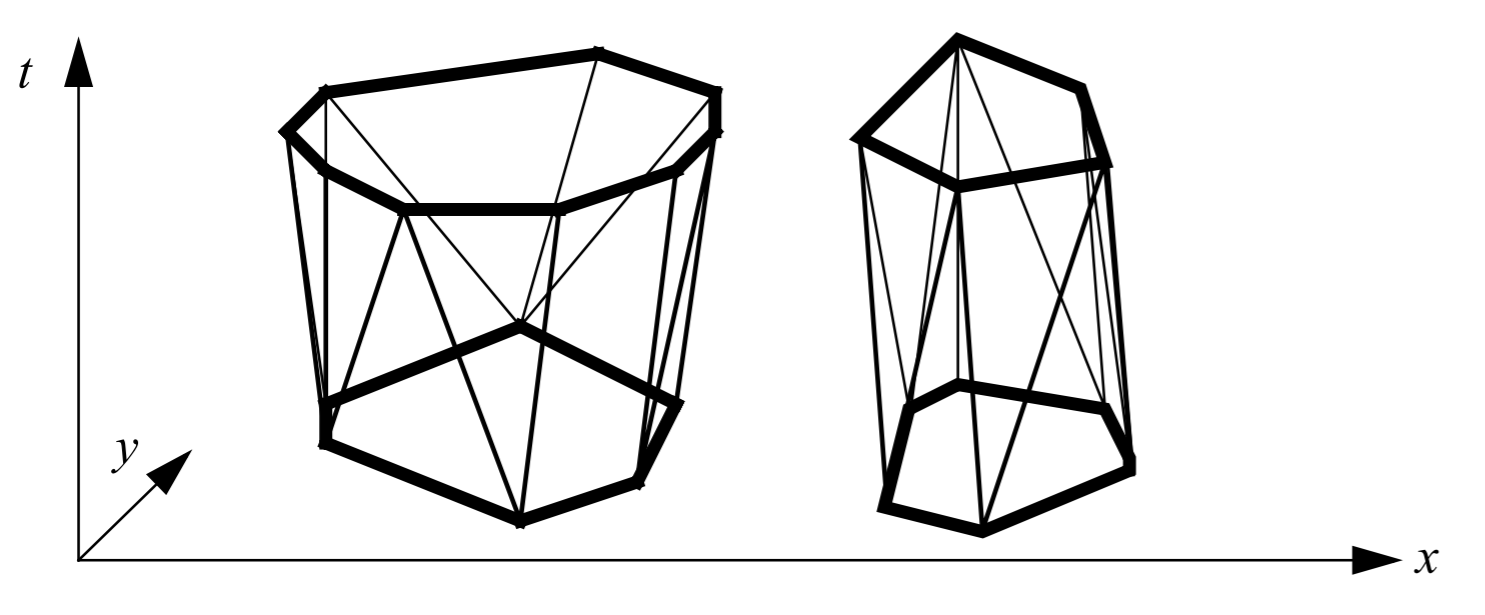
\includegraphics[width=0.75\textwidth]{images/sliced_moving_region.png}
    \caption[Sliced representation of moving regions]{Sliced representation of moving regions \cite{polyhedra}}
    \label{fig:sliced_repr_polygons}
\end{figure}

This sliced representation of moving regions makes use of \textit{moving segments}, which are pairs of \textit{moving points} that are co-planar in 3D space. This definition does not allow segments to rotate, but that can be avoided by representing a rotating segment using two moving segments.

\begin{figure}[h!]
    \centering
    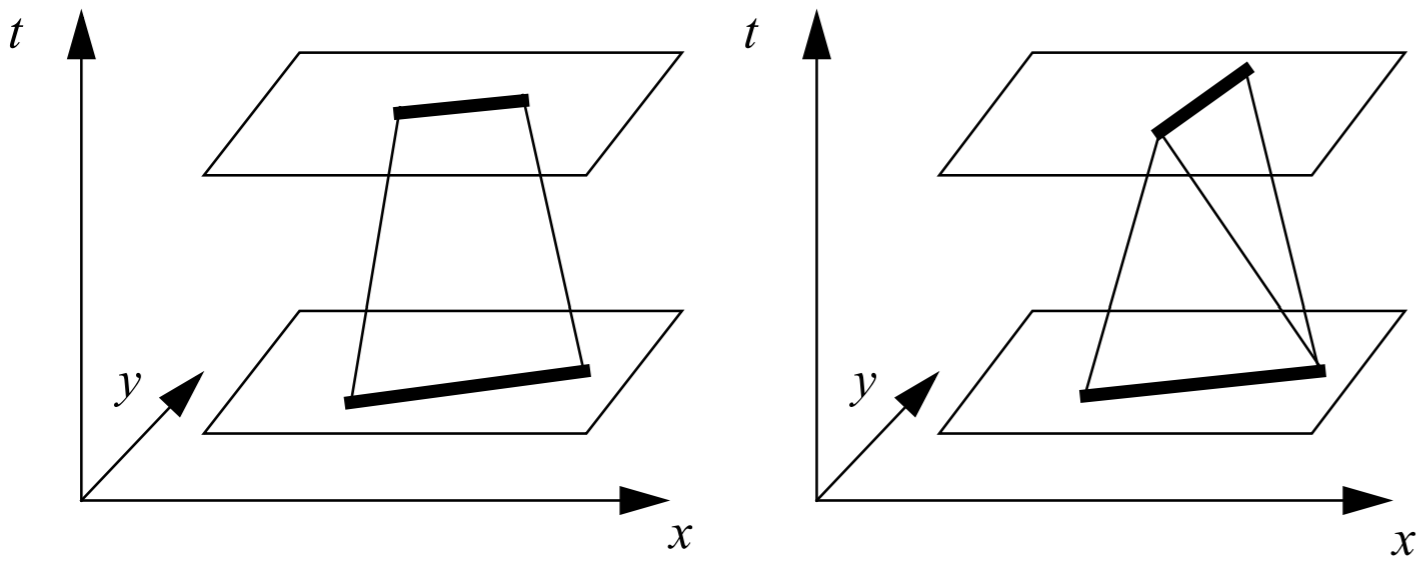
\includegraphics[width=0.75\textwidth]{images/sliced_moving_segments.png}
    \caption[Sliced representation of moving segments]{Sliced representation of moving segments, with rotating segments being represented using 2 distinct moving segments. \cite{polyhedra}}
    \label{fig:sliced_repr_segments}
\end{figure}


To describe the complete movement of a moving region or apply operations on these regions, many of these slices are needed, and this causes storage and efficiency issues. To solve this problem, a polyhedra-based model is described in \cite{polyhedra}, which uses the same moving segments as previously, but computes the operations more efficiently by using the temporal dimension as a third dimension and using 3D geometry to compute the operations. As a result, fewer slices are created than in the previous implementations.

\section{Fixed-Shape Moving Regions}
\label{section:fixed_shape_regions}

Fixed-shape moving regions form another subset of all moving regions and can be used to represent any moving rigid body, such as cars, boats, planes, etc. When the spatial extent of the object is negligible, and the orientation of no importance, the movement of such a body is usually represented by a moving point. When these conditions are not met, however, the movement of the region as a whole has to be analyzed.

The movement of fixed-shape regions can be described much easier than the movement of a deforming region since the only possible transformations are translations and rotations. Theoretically, scaling could be taken into account too, but this case does not seem to have any real-world use case, so it is omitted.

Again, if the region moves in discrete time steps, the technical challenge only concerns the storage space, and here this can be efficiently resolved by storing the moving region as a polygon followed by a list of transformations. This technique is also used when handling the continuous movement of regions and is described below.

When we manage continuous moving regions, we again have to find a way to compute the interpolation efficiently. The previous model for deforming regions relies on moving segments, which are supposed to be non-rotating. This assumption is contradictory to our idea of rotating (and translating) regions, and the larger the rotation of the region is, the worse the interpolation becomes. A good example of this is when a thin rectangle rotates 90 degrees without translating. The interpolation will considerably deform the region, which will at some point become a square, as can be seen in Figure \ref{fig:vertices_interpolation}.

\begin{figure}[h!]
    \centering
    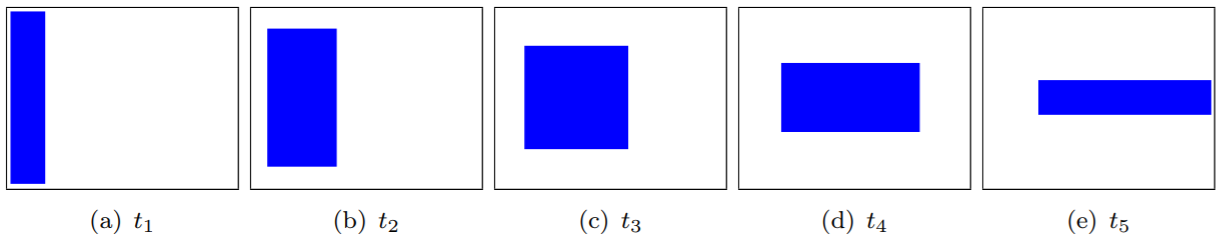
\includegraphics[width=0.75\textwidth]{images/vertices_interpolation.png}
    \caption[Linear interpolation of the vertices of a moving region]{Interpolation of a moving region using linear interpolation between the vertices. \cite{fmregion}}
    \label{fig:vertices_interpolation}
\end{figure}


The reason for this is that the interpolation method does not use the assumptions made on the possible transformations of the polygon. To solve this, a new model is proposed in \cite{fmregion}, which stores the region as a sequence of transformations, and makes use of these transformations to compute the correct interpolation. The resulting fixed-shape moving region is called \lstinline{fmregion} in this paper, and an example of a desired interpolation for this type of region is seen in Figure \ref{fig:fixed_shape_interpolation}.

\begin{figure}[h!]
    \centering
    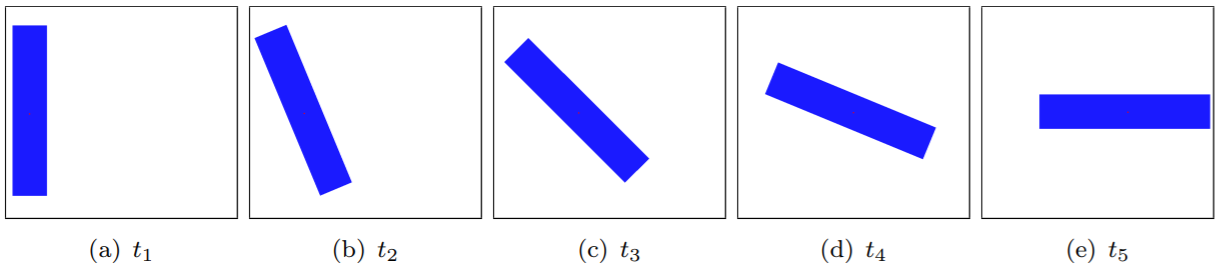
\includegraphics[width=0.75\textwidth]{images/fixed_shape_interpolation.png}
    \caption[Linear interpolation of a fixed-shape moving region]{Interpolation of a moving region using the fixed-shape assumptions. \cite{fmregion}}
    \label{fig:fixed_shape_interpolation}
\end{figure}


The model makes use of a \textit{transformationunit}, which specifies a rotation centre $C$, an initial translation vector $v_0$ and rotation angle $\theta_0$, the vector $v$ and angle $\theta$ representing the transformation, as well as a time interval $[t_s; t_e]$, specifying the start and end instant of the transformation.

\[
    \textit{transformationunit } \mathcal{T}: (C, v_0, v, \theta_0, \theta, t_{s}, t_{e})
\]

An fmregion is thus defined by a single classical region $\mathcal{R}$ and a set of at least one transformation unit $\mathcal{T}$.

\[
    \textit{fmregion} : (\mathcal{R}, \mathcal{T}^{+})
\]

When computing the position of the region at a moment between the start and end instant of a transformation unit, the translation vector, and rotation angle are linearly interpolated, and then the transformation is applied to the initial region to retrieve the position of the region at the correct moment.

Note that the previous definition allows the region to rotate around an arbitrary rotation centre for each transformation unit. This particularity allows the moving region to change rotation centre between two transformation units, which is useful to describe a larger amount of trajectories than if the rotation centre was fixed for all transformations. On the other hand, this also requires the user to input the rotation centre for each transformation, since this cannot be uniquely computed by just seeing the start and end position of the region.

The same paper \cite{fmregion} also describes a few useful algorithms to process moving regions, such as a traversed area function, which computes the union of all places that the region went through during its movement.

\section{3D Moving Regions}
\label{section:3d_regions_intro}

The research articles presented in the two previous sections only focused on moving regions in two dimensions, but of course, we might wonder if 3D moving regions could also be manipulated similarly. Only 3D moving regions of fixed shape fixed-shape will be discussed here. To even just discuss 3D deforming moving regions would require a much larger amount of research.

First of all, it is important to define what we call a 3D region. There is indeed a considerable difference between 3D polygons (polygons with points embedded in 3D space) and 3D polyhedra (3D volumetric objects). In the following, we will define a 3D region as a volumetric geometry, thus representable by a 3D polyhedron.

\begin{figure}[h!]
    \centering
    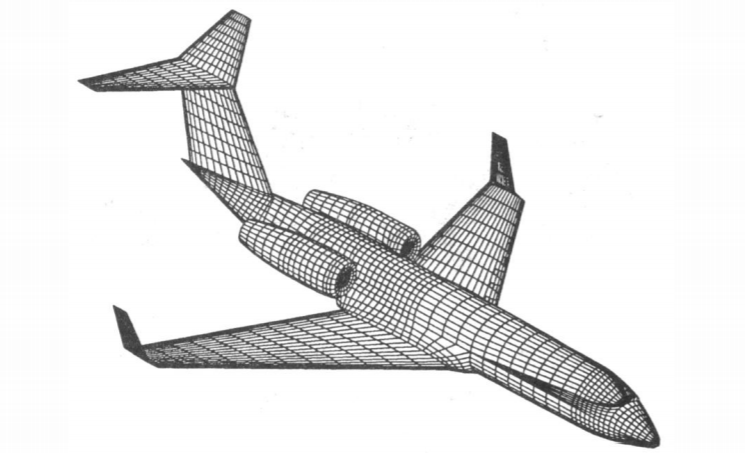
\includegraphics[width=0.75\textwidth]{images/plane_polyhedron.png}
    \caption[Representation of a plane using a 3D polyhedron]{Representation of a plane using a 3D polyhedron \cite{3d_polyhedron}}
    \label{fig:polyhedron}
\end{figure}


Support for 3D geometries is currently extremely restricted in database management systems \cite{3d_geom}. However, PostGIS does support two types of 3D geometries: \textit{Polyhedral Surfaces} and \textit{Triangulated Irregular Network Surfaces} [TIN], which are polyhedral surfaces where every polygon is a triangle. A few 3D functions are also implemented, such as \lstinline{ST_3DClosestPoint} or \lstinline{ST_3DDistance}.

First, let's look at the case where the regions move in discrete time steps. In this case, like previously, the problem of interpolating between two instants does not arise, and the difficulty is reduced to storing the large amount of data that might be present in an efficient manner. 

If we assume fixed-shape regions, we can again use the fact that the only possible transformations are translations and rotations. It is thus sufficient to store the region once as a 3D polyhedron, and then store only the difference in position and orientation for all other positions. This technique is similar to the one described in the previous section, except that the translation and rotation are done in 3D space instead of 2D.

Looking at continuously moving regions, we can apply the same storage idea, and retrieving the position of the region between two stored instants by computing a linear interpolation of the translation, just as was done in 3D, and computing a more advanced interpolation for the 3D rotation, based on \textit{quaternions}.

This interpolation method will be discussed in a later section (Section \ref{section:3d_regions}), but the important part is that it can be done. Storing 3D moving regions of fixed-shape is thus possible, and retrieving the region at any arbitrary instant is too. Implementation of functions that can manipulate and analyze these regions is another issue and is left as future research. 

\chapter{Implementation}
%!TEX root = ../main.tex

\section{Choice of Moving Region Type}
\label{section:region_type_choice}

The previous section describes two different approaches to handle moving regions, each using different assumption, and each having good and bad aspects. Implementing both is not a reasonable goal for this Master thesis, and I thus had to decide which type of region I would chose to implement in MobiltyDB.

The choice was made to focus on implementing a model for manipulating moving regions of fixed-shape, based on the model presented in \cite{fmregion} and described previously. This decision was mostly arbitrary, based on personal preference, but not only. 

MobilityDB already has an underlying structure for the new data types, and this structure has to be preserved as much as possible when implementing a new feature, and this was also a factor in the final decision. The deformable region model uses a \textit{sliced representation} of the movement, whereas MobilityDB uses a \textit{sequence representation} described in \cite{mobilitydb}, so the model would have to be heavily adapted to conform to the MobilityDB structure. Using a sequence representation for storing fixed-shape moving regions seems much more straight forward.

For the rest of the thesis, we can thus assume that we are always talking about regions of fixed-shape, except if explicitly mentioned that we talk about deformable regions.

\section{Representation of Fixed-Shape Moving Regions in MobilityDB}
\label{section:internal_repr}

Now that the choice of the type of region is done, the next challenge is finding a suitable representation for these moving regions in MobilityDB. As said previously, the structure of the system has to be preserved as much as possible, which means that a temporal region type will be required for all four durations: \textit{Instant}, \textit{Instant Set}, \textit{Sequence} and \textit{Sequence Set}. These four types will be called: \textit{tgeometryinst} (for \textit{temporal geometry of instant duration}), \textit{tgeometryi}, \textit{tgeometryseq} and \textit{tgeometrys}.

\subsection{TgeometryInst}
\label{section:internal_repr_inst}

A moving region of instant duration is basically a static region, with an associated timestamp. As said in Section \ref{section:postgis}, the PostGIS type \textit{Geometry(Polygon)} will be used to describe a static region. A tgeometryinst can thus be represented similarly to any other temporal type of instant duration, that is: as a pair of value and timestamp

\[
    'v@t'
\]

, where the value is a PostGIS polygon object, and t is the timestamp. Since only one instant is present, there is no redundancy, and this is the most efficient way to store this type.

\subsection{TgeometryI}
\label{section:internal_repr_i}

As described in section \ref{section:mobilitydb_i}, a temporal value of instant set duration is simply a set of distinct timestamps stored in increasing order of their timestamp. In this case, an additional requirement on the values is present, namely the fact that all regions must be of the same shape.

A simple and naive representation for a tgeometryi is then to store all instants in the set using the previous representation. That is, store for each instant a pair of polygon and timestamp. However, since we have added the extra requirement on the polygons, namely that their shape has to be the same, we are introducing a lot of redundancy in this representation, and the storage is thus not very efficient. \\

Suppose that all the previously mentioned requirements are met, we can store the tgeometryi in a more efficient way, by storing the polygon only once, and storing the subsequent instants using only the transformation with respect to the initial instant. 

Using this representation, a tgeometryi with $n$ instants is written as:

\[
    '\{\mathcal{R}_0@t_0,\ \mathcal{T}_1@t_1,\ \mathcal{T}_2@t_2,\ ..., \ \mathcal{T}_{n-1}@t_{n-1}\}'
\]

, where $\mathcal{R}_0$ is the initial region, and $\mathcal{T}_i$ are the transformation units. \\

Section \ref{section:fixed_shape_regions} describes a possible transformation unit representing a transformation from a start to an end instant. In our case, only the end instant has to be stored, since the start instant will always be represented by the reference region $\mathcal{R}_0$ at time $t_{0}$. Since the start and end timestamp are also already stored elsewhere, namely in the timestamps $t_0$ and $t_i$, we only need to store the rotation center $C$, the translation vector $(v^x,\ v^y)$ and the rotation angle $\theta$ in the transformation unit.

\[
    \mathcal{T}_i: (C_i, v_i^x, v_i^y, \theta_i)
\]

If we want to compute the transformation unit starting from the initial and final polygons, we need to also define a rotation center for all the other parameters to be uniquely defined. For example, if we look at the start and end polygon (dark blue) shown in Figure \ref{fig:center_of_rotation}, multiple transformation units can be defined, all having the same initial and final position, but they differ in their rotation center and the path they take. The blue path has a fixed rotation center at $(3.5,\ 1)$, and there is no translation involved, while the red path uses the centroid of the polygon as rotation center, and involves a translation by 5 units along the x-axis.

\begin{figure}[h!]
    \centering
    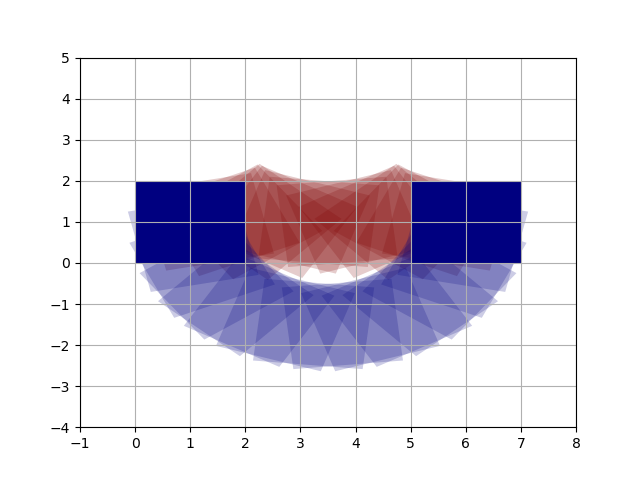
\includegraphics[width=0.75\textwidth]{images/center_of_rotation_importance.png}
    \caption{Importance of the center of rotation for a transformation.}
    \label{fig:center_of_rotation}
\end{figure}


We also know that a temporal instant set is defined only at its instants, and not in between. This means that we only care about the start and end position of a region, but we do not care about the path taken during the transformation. 

Since the decision of the rotation center only changes the path taken by the region during the transformation, the previous observation tells us that we can chose the rotation center arbitrarily when computing the transformation unit. \\

The rotation center takes a certain amount of storage space, and since we just realized that we can chose it arbitrarily, we will define the rotation center of all transformation units as being the centroid of the region at instant $t_0$. With the rotation center fixed, we can save storage space by only storing the translation vector and the rotation angle for each transformation. 

\[
    \mathcal{T}_i: (v_i^x, v_i^y, \theta_i)
\]

Using this representation, we can store a tgeometryi using minimal storage space. The two remaining challenges are: how do we compute a transformation unit starting from an initial and final polygon value, and how do we recompute the position of the region, starting from an initial polygon, and a transformation unit? The solution to these two problems is described in sections \ref{section:compute} and \ref{section:apply}. \\

As a side note, the current implementation recomputes the centroid of the polygon (center of rotation) using the PostGIS function \textit{ST\_Centroid} every time it is needed, but if we later realize that this computation is done often and is not very efficient, we can also compute it once during the input of the moving region, and then store it with the region in the first instant.

\subsection{TgeometrySeq}
\label{section:internal_repr_seq}

A temporal region of sequence duration represents the continuous movement of a region, where the position of the moving region can be retrieved at every instant between the initial and final instant. Here, we thus not only care about the position of the region at the input instants, but we also need to be able to interpolate the region between two defined instants.

As we realized previously, when computing a transformation unit starting from the initial and final position of the polygon, the choice of the rotation center defines the path taken during the movement uniquely. This means that the rotation center will have an impact on the interpolation. \\

One important assumption that was implicitly made for the tgeometryi type, is the fact that a tgeometryseq is input as a list of tgeometryinst. We are thus not getting any extra information other than the snapshots of the regions at specific instants, and, in particular, we do not know what the rotation center is for every transformation. This means that we need to define a rotation center ourselves for the transformations to be well-defined.

Having to define a rotation center ourselves has multiple consequences. First of all, since there is no way to know what the real center of rotation was simply based on the snapshots of the region at the given instants, the only solution we have is to decide on an arbitrary center of rotation. Secondly, since the arbitrary center of rotation will most probably not be the real center of rotation, there will be errors between the real path taken by the region and the interpolated path. \\

Since we know that we have to define an arbitrary center of rotation, the most obvious solution is to take the centroid of the region as the rotation center, since this point is well-defined for all regions and is easy to compute. As you might remember, this is the same solution as for tgeometryi, so we can represent a tgeometryseq in the following way:

\[
    '[\mathcal{R}_0@t_0,\ \mathcal{T}_1@t_1,\ \mathcal{T}_2@t_2,\ ..., \ \mathcal{T}_{n-1}@t_{n-1}]'
\]

, with $\mathcal{T}_i$ being the transformation with respect to $\mathcal{R}_0$:

\[
    \mathcal{T}_i: (v_i^x, v_i^y, \theta_i)
\]

The algorithmic challenges for this data type are the same as for tgeomtryi, with the addition of one problem. This problem is stated in the following way: given a polygon defined at time $t_0$, and two transformation units defined at times $t_i$ and $t_{i+1}$, both defined with respect to the initial polygon, how do we compute the position of the region at any given time $t$, where $t_i < t < t_{i+1}$? The solution to this problem is given in section \ref{section:interpolate}. \\

One last unsolved problem is the fact that the interpolated path does not exactly follow the real path taken by the moving region, when the real rotation center of the moving region is not its centroid. Solving this issue algorithmically would require us to know the real path taken by the moving region and thus the real rotation center, which, as we explained previously, is not possible when we only get snapshots of the region at distinct instants. 

The only solution to this problem without changing the assumptions made, is to give as much snapshots of the region in the input as needed to minimize the difference between interpolated path and the real path. Indeed, we can achieve any arbitrary precision by increasing the amount of instants given in the input between the initial and final position of the region. An example of how giving more instants can increase the precision of the interpolation is shown in figure \note{ref to figure}. \\

\note{Image of better interpolation when using more instants (3 images, 1 with real movement, 1 with only start and end instant, 1 with more instants)}

Here we have a square rotating around a stationary point $(0,\ 0)$. Given only the start and end instant (in red) of the square, the interpolation using the centroid as rotation center would be quite far from the real path taken by the square. Given a few more instants (in blue), the difference between the interpolated path and the real path decreases.

\subsection{TgeometryS}
\label{section:internal_repr_s}

The last type that we have to handle is tgeometrys, which is a temporal geometry of sequence set duration. The input to this type is a list of tgeometryseq. This means that we already receive some of the instants as transformations with respect to the first instant of their sequence.

For this to be a valid tgeometrys, we first need to check the fact that all regions have the same shape. Since this check was already made independently for each sequence when they were created, we thus only need to make sure that the polygons of the first instants of every sequence have the same shape. \\

Assuming that all sequences describe the movement of  polygons of the same shape, we have two possibilities to store this set of sequences. The first possibility is to store every sequence as it was received

\[
    '\{[\mathcal{R}_0^0@t_0^0,\ \mathcal{T}_1^0@t_1^0,\ ...],\ [\mathcal{R}_0^1@t_0^1,\ \mathcal{T}_1^1@t_1^1,\ ...],\ ...\}'
\]

, with every transformation $\mathcal{T}_i^j$, being defined with respect to the region $\mathcal{R}_0^j$ at the start of the sequence.

This solution is easy, since we do not have to do any more preprocessing, but it also has some redundancies, since we know that the first region of each sequence has the same shape. \\

The second possibility is thus to remove the redundancy by replacing the region values of the first instants of all sequences after the first by a transformation value. For all sequences after the first one, we have to compute the transformation of the first instant of the sequence $\mathcal{T}_0^j$ with respect to the first instant of the first sequence of the set $\mathcal{R}_0^0$. All other transformations of the sequence would have to be modified too, to have the start region being the first instant of the first sequence.

The representation would look like this:

\[
    '\{[\mathcal{R}_0^0@t_0^0,\ \mathcal{T}_1^0@t_1^0,\ ...],\ [\mathcal{T}_0^1@t_0^1,\ \mathcal{T}_1^1@t_1^1,\ ...],\ ...\}'
\]

, where every transformation $\mathcal{T}_i^j$, is defined with respect to the region $\mathcal{R}_0^0$ at the start of the first sequence.

This option requires some more preprocessing, but requires less storage space than the previous option. Another disadvantage of this method is the retrieval of a sequence in the set. This operation requires us to re-transform the whole sequence to its input representation if the required sequence is not the first one.

Depending on the use case, the average number of sequences in a set, the average number of instants in each sequence and a few more parameters, either the first option or the second option could prove to be more interesting. \\

The option that has been implemented in practice is the first one, as it seems to be the easiest one to implement, and seems to be implementable using cleaner and less code than the second option. Implementing the second option and comparing their efficiency is left as future research.

\subsection{Rtransform}

In three of the last four types, a transformation unit was used to represent an instant of a moving region more efficiently than by using a polygon. This transformation unit is stored in the database using a new type called \textit{rtransform} (short for \textit{region transformation}). As explained previously, this type only need to store information about the translation vector $(v^x,\ v^y)$ and rotation angle $\theta$ of the final value of the region, since we assume that we know what the start instant is, and we also assume the center of rotation to be the centroid of the region. Internally, all parameters of the rtransform type will be represented using the \textit{double} type.

\[
    \text{rtransform}\ \mathcal{T}: (\text{double}\ v_x,\ \text{double}\ v_y,\ \text{double}\ \theta)
\]

Since we know that rotating by $\theta$ or rotating by $\theta + 2\pi$ gives the same final result, we will add an additional constraint on the rotation angle stored in an rtransform object: $-\pi < \theta \le \pi$. This constraint allows us to compute a unique transformation unit when starting from an initial and final polygon. \\

An rtransform like this always has to be related to a polygon object, usually the polygon stored in the value of the first instant of the sequence, which will be the initial polygon. We can then apply the rtransform as explained in \ref{section:apply} to the start polygon, to retrieve the final polygon. Retrieving the polygon at an instant that is in between two stored instants, will require us to interpolate between two saved transformations to retrieve the final polygon. This interpolation method is explained in section \ref{section:interpolate}.


\section{Utility Functions for Tgeometry and Rtransform types}

Before diving into the implementation of the general MoblityDB functions that have to be adapted to handle moving regions as well as all the types already present, we will first talk about a set of functions specific to the tgeometry and rtransform types.

These functions can be called utility functions, since they are not presented to the user as an SQL function, but they are used in the backend a lot to simplify other functions. Table \ref{table:rtransform_functions} shows a list of these functions with their signature (input and output types).

\begin{table}[h!]
    \centering
    \begin{tabular}[c]{|l|l|} 
    \hline
    \textbf{Functions}  & \textbf{Signature} \\ 
    \hline
    compute             & polygon    x polygon              $\rightarrow$ rtransform \\
    apply               & rtransform x polygon              $\rightarrow$ polygon \\
    \hline
    interpolate         & rtransform x rtransform x double  $\rightarrow$ rtransform \\
    interpolate long    & rtransform x rtransform x double  $\rightarrow$ rtransform \\
    \hline
    combine             & rtransform x rtransform           $\rightarrow$ rtransform \\
    diff                & rtransform x rtransform           $\rightarrow$ rtransform \\
    \hline
    \end{tabular}
    \caption{Utility functions for \textit{rtransform} type}
    \label{table:rtransform_functions}
\end{table}

\subsection{Compute}

The \textit{compute} function takes two polygon values as input and computes the transformation from the first to the second one. For example, taking the two polygons shown below as input, with the red polygon being the first argument and the blue polygon being the second, the resulting rtransform will be $\mathcal{T}:\ ()$ \note{fill in correct rtransform}.

\note{Image of a red and blue polygon}

As said previously the type used to represent a region value is the PostGIS type \textit{Geometry(Polygon)}. This polygon type is defined using rings: one outer ring, and zero or more inner rings defining holes in the polygon. One assumption that we make when recieving the polygons as input is that two polygons of the same shape have their corresponding points defined at the same position in the rings of said polygons. 

The rings are defined as lists of points, with the first and the last points being equal to denote that the ring is closed. Our previous assumption thus sais that the $i$'th point in the list defining the outer ring of the first polygon, has to correspond to the $i$'th point in the list defining the outer ring of the second polygon, after application of the correct transformation.

Essensially this means that the points of the polygons are 'numbered' in the same way. This allows us for example to distinguish a square from its 90 degree rotations.

\note{Image of a square with corners numbered as '1-2-3-4' and '2*-3*-4*-1*', to show that we cannot distinguish the two squared without their numbering}

We can describe the combination of a rotation by $\theta$ around the origin, followed by a translation by $(v^x,\ v^y)$, using a matrix multiplication.

\[
    \begin{bmatrix}
    x' \\
    y' \\ 
    1  \\       
    \end{bmatrix}
    =
    \begin{bmatrix}
    \cos(\theta) & \sin(\theta)  & v^x \\
    \sin(\theta) & -\cos(\theta) & v^y \\ 
    0            & 0             & 1   \\       
    \end{bmatrix}
    *
    \begin{bmatrix}
    x \\
    y \\ 
    1 \\       
    \end{bmatrix}
\]

Using the notation

\[
    \begin{cases}
        a = \cos(\theta) \\
        b = \sin(\theta) \\
        c = v^x          \\
        d = v^y          \\
    \end{cases}
\]

, and by taking the first two points of the outer rings of both input polygons, we have the following list of equations:

\[
    \begin{cases}
        a*x_1 - b*y_1 + c = x_1' \\
        a*y_1 + b*x_1 + d = y_1' \\
        a*x_2 - b*y_2 + c = x_2' \\
        a*y_2 + b*x_2 + d = y_2' \\
    \end{cases}
\]

, with $(x_1, y_1)$ and $(x_2, y_2)$ being the first two points of the first polygon, and $(x_1', y_1')$ and $(x_2', y_2')$ being the corresponding points on the second polygon.

We can then solve these equations for $a$, $b$, $c$ and $d$.

\[
    \begin{cases}
        a = \frac{(x_1' - x_2')*(x_1 - x_2) + (y_1' - y_2')*(y_1 - y_2)}{(x_1 - x_2)^2 + (y_1 - y_2)^2}\\
        b = \frac{(y_1' - y_2')*(x_1 - x_2) - (x_1' - x_2')*(y_1 - y_2)}{(x_1 - x_2)^2 + (y_1 - y_2)^2}\\
        c = x_1' - a*x_1 + b*y_1 \\
        d = y_1' - a*y_1 - b*x_1 \\
    \end{cases}
\]

And finally we can get the parameters of the transformation

\[
    \begin{cases}
        \theta = atan2(b,\ a) \\
        v^x = c \\
        v^y = d \\
    \end{cases}
\]

As said previously, this computes a transformation, wich is the combination of first a rotation $\theta$ applied around the origin, and then a translation $(v^x,\ v^y)$. To use these equations, we thus need the centroid of the first polygon (the center of rotation for this transformation) to be at the origin. To solve this issue, we first compute the centroid of the first region, then translate both regions using the same translation, to have the new centroid of the first region be at the origin. Finally we can use the above equations to compute the parameters of the transformations.

When we also need to verify that both input polygons have the same shape, we can apply this computed transfomation to the start polygon, and compare all corresponding points with the end polygon after the transformation. If the position of two corresponding points differs by more than a given \textit{epsilon}, we can assume that the two regions do not have the same shape.

\subsection{Apply}

This \textit{apply} function does the opposite of the \textit{compute} function. Given an rtransform, and a start polygon, it applies the transformation to retrieve the end polygon. This is done using a PostGIS function called \textit{ST\_Affine}, which applies an affine transformation to the given geometry. 

Applying an affine transformation again means rotating aroung the origin, so we first have to translate the polygon to have its centroid at the origin, then we can apply the given transformation, and finally we apply the inverse of the first translation to get the final polygon.

\subsection{Interpolate}

This function is used when we have a polygon defined at time $t_1$ and another one defined at time $t_2$, and we want to retrieve the position of the polygon at time $t$, where $t_1 < t < t_2$.

If we wanted to interpolate two polygons using linear interpolation between their vertices, we would not keep the fixed-shape aspect of the polygon, as is shown below. For this reason, the interpolation is done on the rtransforms defining the position of the polygon with respect to a certain reference polygon at times $t_1$ and $t_2$.

\note{Show linear interpolation between the vertices of a polygon.}

For example, we have a tgeometryseq with three instants defined at times $t_0$, $t_1$ and $t_2$. 

\[
    '[\mathcal{R}_0@t_0,\ \mathcal{T}_1@t_1,\ \mathcal{T}_2@t_2]'
\]

Suppose now that we want to compute the position of the region at time $t_1 < t < t_2$. To do this, we first apply the \textit{interpolate} function with $\mathcal{T}_1$ and $\mathcal{T}_2$ a arguments, and then apply the resulting rtransform to $\mathcal{R}_0$ to get the result.

The \textit{interpolate} functions takes three input arguments. The first two arguments are the initial and final rtransform values. The third argument is a \textit{ratio} value defined by the timestamp of the resulting rtransform. This ratio is always between 0 and 1, and is computed as follows.

\[
    ratio = \frac{t - t_1}{t_2 - t_1}
\]

Since we assume linear interpolation between the rtransform values, we will simply use linear interpolation to compute the resulting translation value.

\[
    \begin{cases}
        v^x = v_1^x + (v_2^x - v_1^x) * ratio \\
        v^y = v_1^y + (v_2^y - v_1^y) * ratio \\
    \end{cases}
\]

The interpolation of the angle of rotation on the other hand is slightly more complicated. We are still interpolating linearly, but we have to take into account that the angles $-\pi$ and $\pi$ correspond to the same rotation. This means that there are always two possibilities for the interpolation. Either go directly from $\theta_1$ to $\theta_2$ or go from $\theta_1$ to $-\pi$ (if $\theta_1 < \theta_2$) and then from $\pi$ to $\theta_2$. Both are valid interpolations, but one is shorter than the other. The shorter option is the option that will be taken for the interpolation of the angles.

\note{Image of linear axis for the angles and the 2 ways of interpolating}

Any angle of rotation of $-\pi < \theta \le \pi$ can be represented by a point on the unit circle at $(\cos(\theta),\ \sin(\theta))$, which means that going from one angle to the other during the interpolation is the same as moving from one point to the other along the arc of the unit circle. The two possible ways of interpolating angles are thus represented by the two arcs connecting the points, one being longer than the other.

\note{Image of unit circle for the interpolation of angles}

Using this unit circle representation, we can then visualise four different ways of interpolating two angles depending on the values of the two angles. These four cases are shown in figure \note{link to figure}.

\note{figure with 4 cases when interpolating, and an arrow pointing from $\theta_1$ to $\theta_2$ through the smallest arc.}

Computing the interpolated angle is then done using one of the four equations below, depending on in which of the cases shown in \note{link to figure above} we currently are.

\[
    \theta = 
    \begin{cases}
        \text{case 1: } \theta_1 + (\theta_2 - \theta_1)*ratio \\
        \text{case 2: } \theta_2 + (\theta_1 - \theta_2)*(1 - ratio) \\
        \text{case 3: } \theta_1 + (2\pi + \theta_2 - \theta_1)*ratio \\
        \text{case 4: } \theta_2 + (2\pi + \theta_1 - \theta_2)*(1 - ratio) \\
    \end{cases}
\]

Finally, if the resulting angle is larger than $\pi$, we substract $2\pi$ from it to keep the angle between $-\pi$ and $\pi$.

As a last remark, if the difference between the start and end angle is exactly $\pi$, we always interpolate in a counter-clockwise manner. This means that when $\theta_1 < \theta_2$, the interpolation goes through $0$, and otherwise the interpolation goes through $\pi$.

\note{Maybe image of interpolation cases when $\theta_{diff} = \pi$}

\subsection{Interpolate Long}

The \textit{interpolate long} function does the same as the \textit{interpolate} function, except that during the interpolation of the angles, it always takes the longest arc instead of the smallest. This function will be useful in section \note{link to normalization section}, when normalizing a tgeometryseq.

\subsection{Combine}

The \textit{combine} function essentially does an addition of two rtransform value. With the input rtransform objects being written as $(v_1^x,\ v_1^y,\ \theta_1)$ and $(v_2^x,\ v_2^y,\ \theta_2)$, the resulting rtransform is computed as:

\begin{align*}
        & v^x = v_1^x + v_2^x \\
        & v^y = v_1^y + v_2^y \\
        & \theta = 
        \begin{cases}
            \theta_1 + \theta_2 - 2\pi,\ \text{if } \pi < \theta_1 + \theta_2 \\
            \theta_1 + \theta_2 + 2\pi,\ \text{if } \theta_1 + \theta_2 \le -\pi \\
            \theta_1 + \theta_2,\ \text{otherwise}
        \end{cases}
\end{align*}

This function is used when we need to change the start/reference region of the rtransform, for example when we need to merge two tgeometryi. 

\begin{flalign*}
    & \text{merge(}\{\mathcal{R}_0@t_0,\ \mathcal{T}_1@t_1\},\ \{\mathcal{R}_0'@t_2,\ \mathcal{T}_1'@t_3\}) &&\\
    & \text{-- -- }\ '\{\mathcal{R}_0@t_0,\ \mathcal{T}_1@t_1,\ \mathcal{T}_2@t_2,\ \mathcal{T}_3@t_3\}'\ \text{-- --} &&\\
\end{flalign*}

In this case, computing $\mathcal{T}_3$ requires us to \textit{combine} $\mathcal{T}_1'$ and the newly computed $\mathcal{T}_2$.

\subsection{Diff}

The \textit{diff} function is similar to the compute fuction, except that it does the difference between the first and the second input argument, instead of doing an addition.

\begin{align*}
        & v^x = v_2^x - v_1^x \\
        & v^y = v_2^y - v_1^y \\
        & \theta = 
        \begin{cases}
            \theta_2 - \theta_1 - 2\pi,\ \text{if } \pi < \theta_2 - \theta_1 \\
            \theta_2 - \theta_1 + 2\pi,\ \text{if } \theta_2 - \theta_1 \le -\pi \\
            \theta_2 - \theta_1,\ \text{otherwise}
        \end{cases}
\end{align*}

When we want to know what the transformation is between two instants, when both instants are saved as rtransforms relative to a third instant, we can use simply do the difference between the rtransform of the final instant and the rtransform of the initial instant to get the result.

For example, if we have a tgeometryi with 3 instants $'\{\mathcal{R}_0@t_0,\ \mathcal{T}_1@t_1,\ \mathcal{T}_2@t_2\}'$, and we want to get the transformation to go from the second instant to the third, we can apply $\textit{diff}(\mathcal{T}_2,\ \mathcal{T}_1)$.
%!TEX root = ../main.tex

\section{Implementation of MobilityDB Functions}
\label{section:general_functions}

The main focus of this master thesis is extending MobilityDB by adding a new type to represent moving regions and by implementing a set of functions to input, manipulate and output this new type. In Section \ref{section:mobilitydb_functions}, different types of functions and operators are presented, and most of these functions are polymorphic, meaning that they accept different input types and that their output depends on these input types. The next section lists and describes most of these functions, and explains how they are used to manipulate the \lstinline+tgeometry+ type.

\subsection{Type Declaration Functions and Parameters}
\label{section:type_declaration}

When defining a new SQL type, 2 functions have to be declared, and a few other functions and parameters are optional. The two required functions are \lstinline{input} and \lstinline{output}, converting a \lstinline{cstring} (C string type) to the newly declared type and back. The optional functions and parameters are used to declare the internal storage length of the type, the storage alignment in bytes, input/out to and from byte format, type modifier specification, and more.

As explained previously, two new types have been added to MobilityDB: \lstinline{rtransform} and \lstinline{tgeometry}. Four variations of the \lstinline+tgeometry+ type (\lstinline{tgeometryinst}, \lstinline{tgeometryi}, \lstinline{tgeometryseq} and \lstinline{tgeometrys}) are also present at the C-level, but only these two top-level types are exposed at the SQL level. Table \ref{table:rtransform_type_declaration} lists the declared parameters and functions for the \lstinline+rtransform+ type, and Table \ref{table:tgeometry_type_declaration} described the \lstinline+tgeometry+ type.

\begin{table}[htb]
    \centering
    \begin{tabularx}{\textwidth}{|l|l|X|}
    \hline
    \textbf{Parameter}  & \textbf{Value}        & \textbf{Description} \\ 
    \hline
    \lstinline+internal length+     & 24                    & Internal storage length in bytes. \\
    \hline
    \lstinline+alignment+           & \lstinline+double+                & Storage alignment of the type. \\
    \hline
    \multicolumn{2}{|l|}{\textbf{Function}}     & \textbf{Description} \\ 
    \hline
    \multicolumn{2}{|l|}{\lstinline+input+}     & Conversion from \lstinline{cstring} to \lstinline{rtransform} type \\
    \hline
    \multicolumn{2}{|l|}{\lstinline+output+}    & Conversion from \lstinline{rtransform} to \lstinline{cstring} type \\
    \hline
    \multicolumn{2}{|l|}{\lstinline+receive+}               & Conversion from \lstinline{bytea} to \lstinline{rtransform} type \\
    \hline
    \multicolumn{2}{|l|}{\lstinline+send+}                  & Conversion from \lstinline{rtransform} to \lstinline{bytea} type \\
    \hline
    \end{tabularx}
    \caption{Declared parameters and functions for the \lstinline{rtransform} type}
    \label{table:rtransform_type_declaration}
\end{table}

The \lstinline+rtransform+ type stores three double (8-byte) values, two for the translation and one for the rotation, and has thus a fixed length of 24 bytes. Since values of this type will never be store alone, but always as part of a \lstinline+tgeometry+ value, the storage strategy does not need to be declared. During the input from a string, we make sure that the value for the rotation is between $-\pi$ and $\pi$. The output as a string is formatted as

\[
    \text{"RTransform(}\theta,\ v_x,\ v_y{)"}, 
\]
where all three values are written with up to 15 decimal digits. The binary representation is simply a list of three doubles in the same order as in the string representation.

\begin{table}[htb]
    \centering
    \begin{tabularx}{\textwidth}{|l|l|X|}
    \hline
    \textbf{Parameter}  & \textbf{Value}        & \textbf{Description} \\ 
    \hline
    \lstinline+internal length+     & \lstinline+variable+              & Internal storage length of the type in bytes. \\
    \hline
    \lstinline+storage+             & \lstinline+extended+              & Storage strategy of the type. \\
    \hline
    \lstinline+alignment+           & \lstinline+double+                & Storage alignment of the type. \\
    \hline
    \multicolumn{2}{|l|}{\textbf{Function}}     & \textbf{Description} \\ 
    \hline
    \multicolumn{2}{|l|}{\lstinline+input+}     & Conversion from \lstinline{cstring} to \lstinline{tgeometry} type \\
    \hline
    \multicolumn{2}{|l|}{\lstinline+output+}    & Conversion from \lstinline{tgeometry} to \lstinline{cstring} type \\
    \hline
    \multicolumn{2}{|l|}{\lstinline+receive+}   & Conversion from \lstinline{bytea} to \lstinline{tgeometry} type \\
    \hline
    \multicolumn{2}{|l|}{\lstinline+send+}      & Conversion from \lstinline{tgeometry} to \lstinline{bytea} type \\
    \hline
    \end{tabularx}
    \caption{Declared parameters and functions for the \lstinline{tgeometry} type}
    \label{table:tgeometry_type_declaration}
\end{table}

The \lstinline+tgeometry+ type contains PostGIS polygons (which are of variable length) and can have an arbitrary number of defined instants, so it must be defined as variable-length. Since the type is variable in length, the \lstinline{plain} storage strategy, storing the values in-line without compression, cannot be used. The \lstinline{extended} strategy is thus used to compress large values, and even move them out of the main table if the value is still too large.

The string representation of the \lstinline+tgeometry+ types depends on the duration of the value as described in Section \ref{section:mobilitydb} (instant, instant set, ...), and represents the values of the instants as PostGIS polygon types. These conversion functions from and to a string are defined together with the conversion functions from and to a byte list.

\subsection{Constructors}
\label{section:constructors}

Four different constructors exist for \lstinline+tgeometry+ types, one for each duration.

\begin{table}[htb]
    \centering
    \begin{tabularx}{\textwidth}{|l|X|}
    \hline
    \textbf{Function}   & \textbf{Signature} \\ 
    \hline
    \lstinline+tgeometryinst+       & \lstinline+geometry(Polygon)+ $\times$ \lstinline+timestamptz+ $\rightarrow$ \lstinline+tgeometry(Instant)+ \\
    \hline
    \lstinline+tgeometryi+          & \lstinline+array tgeometry(Instant)+ $\rightarrow$ \lstinline+tgeometry(Instant Set)+ \\
    \hline
    \lstinline+tgeometryseq+        & \lstinline+array tgeometry(Instant)+ $\times$ \lstinline+lower inclusive+ $\times$ \lstinline+upper inclusive+ $\times$ \lstinline+linear+ $\rightarrow$ \lstinline+tgeometry(Sequence)+ \\
    \hline
    \lstinline+tgeometrys+          & \lstinline+array tgeometry(Sequence)+ $\rightarrow$ \lstinline+tgeometry(Sequence Set)+ \\
    \hline
    \end{tabularx}
    \caption{Constructor functions}
    \label{table:constructor_funcs}
\end{table}

When creating a \lstinline+tgeometryinst+, the input geometry is checked to make sure that it is a 2D polygon. Both the instant set and sequence constructors receive an array of \lstinline+tgeometryinst+ as input, while the sequence set constructor requires an array of \lstinline+tgeometryseq+. Different checks are done to make sure that this input array corresponds to a correct temporal geometry.

First of all, when creating an instance set or a sequence, the usual timestamp checks are done, meaning that the instants must have strictly increasing timestamps. Lastly, the regions are compared with one another, to make sure that they have the same shape.

This comparison between regions is done in two steps. A first quick check compares the number of inner rings of the polygons and if both polygons have the same number of rings, it compares the number of points on each ring. If two polygons pass this check, the transformation between the two polygons is computed from the first two points of the outer ring of both polygons, and the transformation is then applied to one of the polygons. Only polygons where the corresponding points are close enough to each other (their distance is smaller than a fixed $\epsilon$) after the transformation are considered fixed-shape. Figure \ref{fig:constr_checks} shows examples of polygons that fail the first test (a), pass the first test, but fail the second (b), or pass all tests because they are indeed fixed-shape (c).

\begin{figure}[h!]
    \centering
    \begin{subfigure}{.3\textwidth}
        \centering
        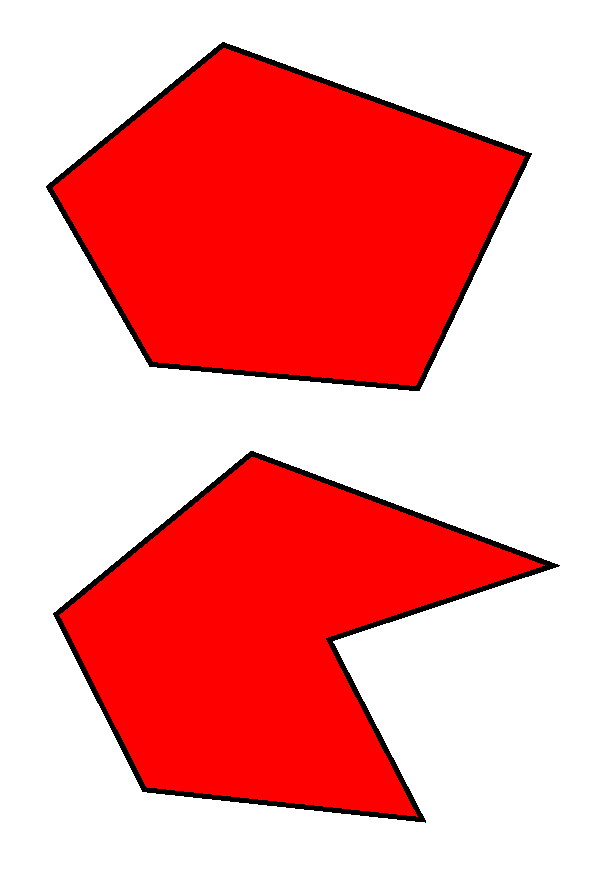
\includegraphics[width=\textwidth]{images/fail_first_test.pdf}
        \caption{Different number of vertices}
    \end{subfigure}
    \hfill
    \begin{subfigure}{.3\textwidth}
        \centering
        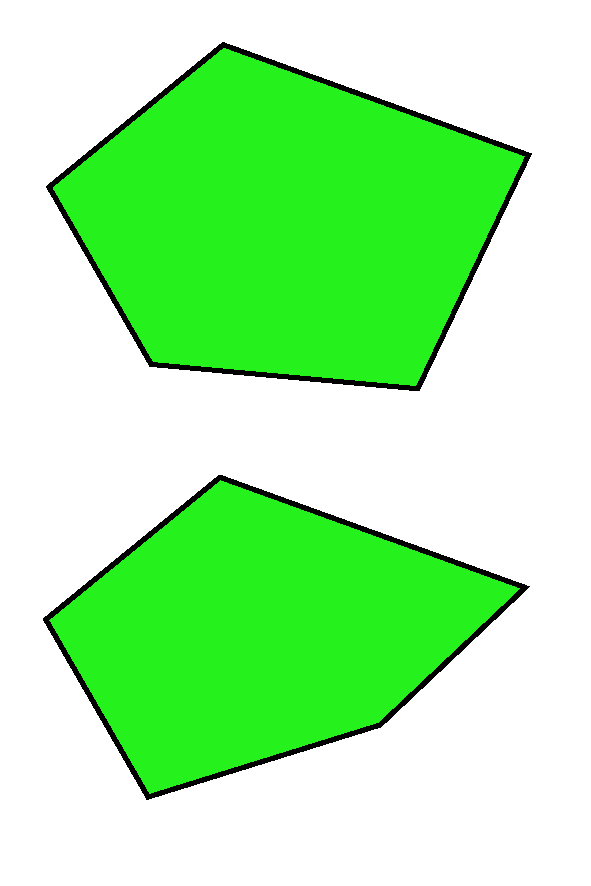
\includegraphics[width=\textwidth]{images/fail_second_test.pdf}
        \caption{Different shape}
    \end{subfigure}
    \hfill
    \begin{subfigure}{.3\textwidth}
        \centering
        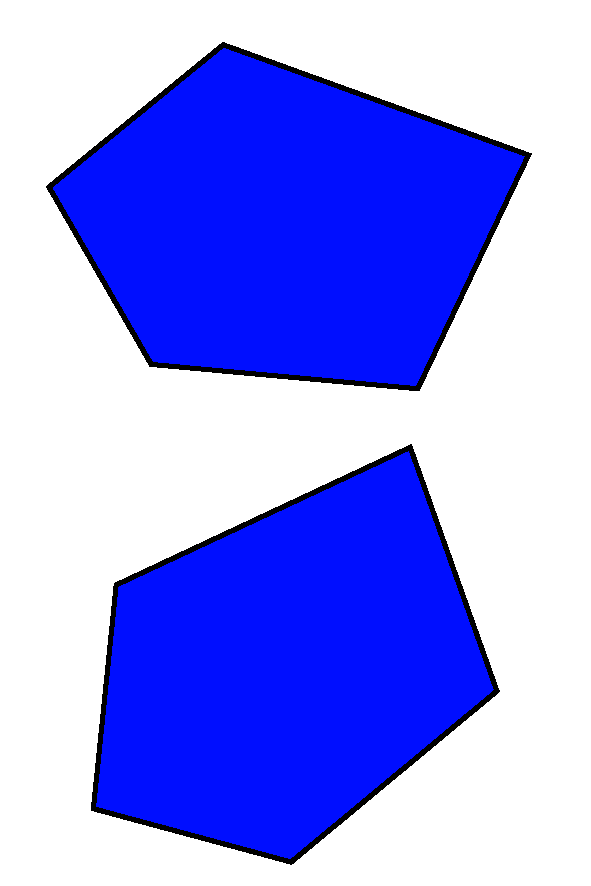
\includegraphics[width=\textwidth]{images/pass_all_tests.pdf}
        \caption{Same shape, only transformed}
    \end{subfigure}
    \caption{Polygons failing or passing the different constructor checks}
    \label{fig:constr_checks}
\end{figure}

If all polygons are indeed fixed-shape, the input array is accepted and saved using the representation described in Sections \ref{section:internal_repr_i} and \ref{section:internal_repr_seq}.

The sequence constructor has three additional parameters. The first two specify if the start and end instant are inclusive or not and by default both are considered inclusive. The last parameter specifies the interpolation strategy for the sequence, either linear or stepwise. The sequence set constructor has checks similar to the two previous ones, but since the input durations are already assumed to be sequences, only the comparisons between distinct sequences have to be done. During these comparisons, checks are done to assure continuously increasing timestamps, and fixed-shape polygons across the whole sequence set.

Every \lstinline+tgeometry+ instance of either instant set, sequence or sequence set duration also computes and saves a bounding box used for optimization purposes. Section \ref{section:bbox_funcs} lists a few bounding-box specific functions, and Section \ref{section:bbox} explains how these bounding boxes can be computed. Temporal points of sequence and sequence set duration also save a \textit{trajectory}, which is also used to optimize a few functions. The polygon equivalent of this trajectory is the \textit{traverser area} of the polygon. The computation of the traversed area of a moving region is discussed in Section \ref{section:traversed_area}.

Lastly, the arrays of instants and sequences stored are normalized during the input process to allow for efficient comparisons later on. This normalization is necessary to ensure that identical paths have the same internal representation. This topic is further discussed in Section \ref{section:normalization}.

\subsection{Transformation Functions}
\label{section:transformation_funcs}

Table \ref{table:transformation_funcs} lists the transformations functions that can be applied to \lstinline+tgeometry+ objects. The first four transformation functions are used to change the duration of a temporal geometry. These transformations are only possible when the correct number of instants and/or sequences are present in the input \lstinline+tgeometry+. For example, for a temporal geometry to be transformed into a \lstinline+tgeometryinst+, it must contain a single instant. Transforming into an instant set from a sequence set is only possible if every sequence in the set contains a single instant. The six possible transformations are listed below.

\begin{itemize}
    \item \lstinline+Instant+ $'\mathcal{R}@t'$ $\leftrightarrow$ \lstinline+Instant Set+ $'\{\mathcal{R}@t\}'$
    \item \lstinline+Instant+ $'\mathcal{R}@t'$ $\leftrightarrow$ \lstinline+Sequence+ $'[\mathcal{R}@t]'$
    \item \lstinline+Instant+ $'\mathcal{R}@t'$ $\leftrightarrow$ \lstinline+Sequence Set+ $'\{[\mathcal{R}@t]\}'$
    \item \lstinline+Instant Set+ $'\{\mathcal{R}@t\}'$ $\leftrightarrow$ \lstinline+Sequence+ $'[\mathcal{R}@t]'$
    \item \lstinline+Instant Set+ $'\{\mathcal{R}_0@t_0,\ ...,\ \mathcal{R}_n@t_n\}'$ $\leftrightarrow$ \lstinline+Sequence Set+ $'\{[\mathcal{R}_0@t_0],\ ...,\ [\mathcal{R}_n@t_n]\}'$
    \item \lstinline+Sequence+ $'[\mathcal{R}_0@t_0,\ ...,\ \mathcal{R}_n@t_n]'$ $\leftrightarrow$ \lstinline+Sequence Set+ $'\{[\mathcal{R}_0@t_0,\ ...,\ \mathcal{R}_n@t_n]\}'$
\end{itemize}

Next to changing their duration, temporal geometries can also be transformed by appending a new instant to the end or by merging two temporal geometries, during which similar checks as in the constructors are applied.

\begin{table}[htb]
    \centering
    \begin{tabularx}{\textwidth}{|l|X|}
    \hline
    \textbf{Function}   & \textbf{Signature} \\ 
    \hline
    \lstinline+tgeometryinst+       & \lstinline+tgeometry+ $\rightarrow$ \lstinline+tgeometry(Instant)+ \\
    \hline
    \lstinline+tgeometryi+          & \lstinline+tgeometry+ $\rightarrow$ \lstinline+tgeometry(Instant Set)+ \\
    \hline
    \lstinline+tgeometryseq+        & \lstinline+tgeometry+ $\rightarrow$ \lstinline+tgeometry(Sequence)+ \\
    \hline
    \lstinline+tgeometrys+          & \lstinline+tgeometry+ $\rightarrow$ \lstinline+tgeometry(Sequence Set)+ \\
    \hline
    \hline
    \lstinline+appendInstant+       & \lstinline+tgeometry+ $\times$ \lstinline+tgeometry(Instant)+ $\rightarrow$ \lstinline+tgeometry+ \\
    \hline
    \lstinline+merge+               & \lstinline+tgeometry+ $\times$ \lstinline+tgeometry+ $\rightarrow$ \lstinline+tgeometry+ \\
    \hline
    \lstinline+merge+               & \lstinline+array tgeometry+ $\rightarrow$ \lstinline+tgeometry+ \\
    \hline
    \end{tabularx}
    \caption{Transformation functions}
    \label{table:transformation_funcs}
\end{table}

\subsection{Accessors}
\label{section:accessors}

A large list of accessor functions exists to retrieve the duration, memory size, individual values, instants, timestamps and more. (Table \ref{table:accessor_funcs})

\begin{table}[htb]
    \centering
    \begin{tabularx}{\textwidth}{|l|X|}
    \hline
    \textbf{Function}   & \textbf{Signature} \\ 
    \hline
    \lstinline+duration+            & \lstinline+tgeometry+ $\rightarrow$ \lstinline+text+\\
    \hline
    \lstinline+interpolation+       & \lstinline+tgeometry+ $\rightarrow$ \lstinline+text+\\
    \hline
    \lstinline+memSize+             & \lstinline+tgeometry+ $\rightarrow$ \lstinline+integer+ \\
    \hline
    \lstinline+getValue+            & \lstinline+tgeometry(Instant)+ $\rightarrow$ \lstinline+geometry(Polygon)+ \\
    \hline
    \lstinline+startValue+          & \lstinline+tgeometry+ $\rightarrow$ \lstinline+geometry(Polygon)+ \\
    \hline
    \lstinline+endValue+            & \lstinline+tgeometry+ $\rightarrow$ \lstinline+geometry(Polygon)+ \\
    \hline
    \lstinline+getTimestamp+        & \lstinline+tgeometry(Instant)+ $\rightarrow$ \lstinline+timestamptz+ \\
    \hline
    \lstinline+getTime+             & \lstinline+tgeometry+ $\rightarrow$ \lstinline+periodset+ \\
    \hline
    \lstinline+timespan+            & \lstinline+tgeometry+ $\rightarrow$ \lstinline+interval+ \\
    \hline
    \lstinline+shift+               & \lstinline+tgeometry+ $\rightarrow$ \lstinline+tgeometry+ \\
    \hline
    \lstinline+num*+                & \lstinline+tgeometry+ $\rightarrow$ \lstinline+integer+ \\
    \hline
    \lstinline+start*+              & \lstinline+tgeometry+ $\rightarrow$ \lstinline+*+ \\
    \hline
    \lstinline+end*+                & \lstinline+tgeometry+ $\rightarrow$ \lstinline+*+ \\
    \hline
    \lstinline+*N+                  & \lstinline+tgeometry+ $\times$ \lstinline+integer+ $\rightarrow$ \lstinline+*+ \\
    \hline
    \lstinline+*s+                  & \lstinline+tgeometry+ $\rightarrow$ \lstinline+array *+ \\
    \hline
    \end{tabularx}
    \caption{Accessor functions}
    \label{table:accessor_funcs}
\end{table}

\lstinline{Duration} returns one of $\{$\lstinline{"Instant"}, \lstinline{"Instant Set"}, \lstinline{"Sequence"}, \lstinline{"Sequence Set"}$\}$, \lstinline{interval} returns either \lstinline{"Discrete"} for instants and instant set, or one of $\{$\lstinline{"Linear"}, \lstinline{"Stepwise"}$\}$ for sequences and sequence sets, and \lstinline{memsize} returns the internal memory size in bytes.

Other accessor functions are defined to retrieve individual values, timestamps or sequences from the temporal geometry. In Table \ref{table:accessor_funcs}, all functions containing the symbol '*' are part of a set of functions returning a certain type of element. These functions return the number of that element in the \lstinline+tgeometry+, the first, last or Nth element, and an array containing all elements respectively. This set is defined for the \lstinline{Timestamp}, \lstinline{Instant} and \lstinline{Sequence} elements. A complete list of these functions can be found in Appendix \ref{appendix:complete_funct_tables}.

\subsection{Always/Ever Comparison}
\label{section:always_ever}

These functions and operators compare a temporal geometry with a fixed region value (Polygon) and return the result of the ever equals (\lstinline+ever_eq+), always equals (\lstinline+always_eq+), ever not equals (\lstinline+ever_ne+) or always not equals (\lstinline+always_ne+) comparisons. \\

\begin{table}[h!]
    \centering
    \begin{tabularx}{\textwidth}{|l|l|X|}
    \hline
    \textbf{Function}   & \textbf{Operator} & \textbf{Signature} \\
    \hline
    \lstinline+ever_eq+    & \lstinline+?=+      & \lstinline+tgeometry+ $\times$ \lstinline+geometry(Polygon)+ $\rightarrow$ \lstinline+boolean+ \\
    \hline
    \lstinline+always_eq+  & \lstinline+\%=+     & \lstinline+tgeometry+ $\times$ \lstinline+geometry(Polygon)+ $\rightarrow$ \lstinline+boolean+ \\
    \hline
    \lstinline+ever_ne+    & \lstinline+\&<>+    & \lstinline+tgeometry+ $\times$ \lstinline+geometry(Polygon)+ $\rightarrow$ \lstinline+boolean+ \\
    \hline
    \lstinline+always_ne+  & \lstinline+\%<>+    & \lstinline+tgeometry+ $\times$ \lstinline+geometry(Polygon)+ $\rightarrow$ \lstinline+boolean+ \\
    \hline
    \end{tabularx}
    \caption{Always/Ever comparison functions and operators}
    \label{table:always_ever_funcs}
\end{table}

\subsection{Restriction and Difference Functions}
\label{section:restriction_and_difference}

These functions are used to restrict a temporal geometry to a given value (restriction functions), or to the complement of that value (difference functions). The given value can range from a single region (Polygon) value to a timestamp, or even a set of period values. The full set of restriction functions is listed in Table \ref{table:restriction_funcs}, and Table \ref{table:diff_funcs} lists the difference functions.

\begin{table}[h!]
    \centering
    \begin{tabularx}{\textwidth}{|l|X|}
    \hline
    \textbf{Function}   & \textbf{Signature} \\ 
    \hline
    \lstinline+atValue+             & \lstinline+tgeometry+ $\times$ \lstinline+geometry+ $\rightarrow$ \lstinline+tgeometry+\\
    \hline
    \lstinline+atValues+            & \lstinline+tgeometry+ $\times$ \lstinline+array geometry+ $\rightarrow$ \lstinline+tgeometry+\\
    \hline
    \lstinline+atTimestamp+         & \lstinline+tgeometry+ $\times$ \lstinline+timestamptz+ $\rightarrow$ \lstinline+tgeometry+ \\
    \hline
    \lstinline+atTimestampSet+      & \lstinline+tgeometry+ $\times$ \lstinline+timestampset+ $\rightarrow$ \lstinline+tgeometry+ \\
    \hline
    \lstinline+atPeriod+            & \lstinline+tgeometry+ $\times$ \lstinline+period+ $\rightarrow$ \lstinline+tgeometry+ \\
    \hline
    \lstinline+atPeriodSet+         & \lstinline+tgeometry+ $\times$ \lstinline+periodset+ $\rightarrow$ \lstinline+tgeometry+ \\
    \hline
    \end{tabularx}
    \caption{Restriction functions}
    \label{table:restriction_funcs}
\end{table}

For example, if we want to remove the data in a temporal geometry between to given timestamps, we can use the \lstinline{minusPeriod} function with as second argument a period starting at the first and ending at the second timestamp.

\begin{table}[h!]
    \centering
    \begin{tabularx}{\textwidth}{|l|X|}
    \hline
    \textbf{Function}   & \textbf{Signature} \\ 
    \hline
    \lstinline+minusValue+             & \lstinline+tgeometry+ $\times$ \lstinline+geometry+ $\rightarrow$ \lstinline+tgeometry+\\
    \hline
    \lstinline+minusValues+            & \lstinline+tgeometry+ $\times$ \lstinline+array geometry+ $\rightarrow$ \lstinline+tgeometry+\\
    \hline
    \lstinline+minusTimestamp+         & \lstinline+tgeometry+ $\times$ \lstinline+timestamptz+ $\rightarrow$ \lstinline+tgeometry+ \\
    \hline
    \lstinline+minusTimestampSet+      & \lstinline+tgeometry+ $\times$ \lstinline+timestampset+ $\rightarrow$ \lstinline+tgeometry+ \\
    \hline
    \lstinline+minusPeriod+            & \lstinline+tgeometry+ $\times$ \lstinline+period+ $\rightarrow$ \lstinline+tgeometry+ \\
    \hline
    \lstinline+minusPeriodSet+         & \lstinline+tgeometry+ $\times$ \lstinline+periodset+ $\rightarrow$ \lstinline+tgeometry+ \\
    \hline
    \end{tabularx}
    \caption{Difference functions}
    \label{table:diff_funcs}
\end{table}

\subsection{Comparison Operators}
\label{section:comparison_funcs}

A set of comparison operators is defined in PostgreSQL, and they have been extended to accept arguments of type temporal geometry. In practice, only the equals (\lstinline+=+) and not equals (\lstinline+<>+) operators are useful for real-world applications, but the other operators are used internally to create B-tree indexes on the \lstinline+tgeometry+ type.

\begin{table}[h!]
    \centering
    \begin{tabularx}{\textwidth}{|l|l|X|}
    \hline
    \textbf{Function}   & \textbf{Operator} & \textbf{Signature} \\
    \hline
    \lstinline+tgeometry_lt+    & \lstinline+<+    & \lstinline+tgeometry+ $\times$ \lstinline+tgeometry+ $\rightarrow$ \lstinline+boolean+ \\
    \hline
    \lstinline+tgeometry_le+    & \lstinline+<=+   & \lstinline+tgeometry+ $\times$ \lstinline+tgeometry+ $\rightarrow$ \lstinline+boolean+ \\
    \hline
    \lstinline+tgeometry_eq+    & \lstinline+=+    & \lstinline+tgeometry+ $\times$ \lstinline+tgeometry+ $\rightarrow$ \lstinline+boolean+ \\
    \hline
    \lstinline+tgeometry_ne+    & \lstinline+<>+   & \lstinline+tgeometry+ $\times$ \lstinline+tgeometry+ $\rightarrow$ \lstinline+boolean+ \\
    \hline
    \lstinline+tgeometry_ge+    & \lstinline+>=+   & \lstinline+tgeometry+ $\times$ \lstinline+tgeometry+ $\rightarrow$ \lstinline+boolean+ \\
    \hline
    \lstinline+tgeometry_gt+    & \lstinline+>+    & \lstinline+tgeometry+ $\times$ \lstinline+tgeometry+ $\rightarrow$ \lstinline+boolean+ \\
    \hline
    \lstinline+tgeometry_cmp+   &                  & \lstinline+tgeometry+ $\times$ \lstinline+tgeometry+ $\rightarrow$ \lstinline+integer+ \\
    \hline
    \end{tabularx}
    \caption{Comparison functions and operators}
    \label{table:comparison_funcs}
\end{table}

\subsection{Temporal Comparison Operators}
\label{section:temporal_comparison}

The previous equality and inequality operators returned a single boolean value, but we might also be interested in knowing when two temporal geometries are equal or when they differ as a function of time. The following two operators return a temporal bool representing the result over time of the equality or inequality operator on the input values.

\begin{table}[h!]
    \centering
    \begin{tabularx}{\textwidth}{|l|l|X|}
    \hline
    \textbf{Function}   & \textbf{Operator} & \textbf{Signature} \\
    \hline
    \lstinline+tgeo_eq+    & \lstinline+\#=+   & \lstinline+\{tgeometry, geometry(Polygon)\}+ $\times$ \lstinline+\{tgeometry, geometry(Polygon)\}+ $\rightarrow$ \lstinline+tbool+ \\
    \hline
    \lstinline+tgeo_ne+    & \lstinline+\#<>+  & \lstinline+\{tgeometry, geometry(Polygon)\}+ $\times$ \lstinline+\{tgeometry, geometry(Polygon)\}+ $\rightarrow$ \lstinline+tbool+ \\
    \hline
    \end{tabularx}
    \caption{Temporal comparison functions and operators}
    \label{table:temporal_comparison_funcs}
\end{table}

\subsection{Spatial Functions}
\label{section:spatial_funcs}

As has been done for the temporal points previously in MobilityDB (briefly described in Section \ref{section:mobilitydb_functions}), multiple spatial functions similar to those defined in PostGIS are exposed. 

Table \ref{table:spatial_funcs} shows a non-exhaustive list of spatial functions that can be applied to the \lstinline+tgeometry+ type.

\begin{table}[h!]
    \centering
    \begin{tabularx}{\textwidth}{|l|X|}
    \hline
    \textbf{Function}   & \textbf{Signature} \\ 
    \hline
    \lstinline+traversed_area+      & \lstinline+tgeometry+ $\rightarrow$ \lstinline+geometry(Polygon)+\\
    \hline
    \lstinline+centroid+            & \lstinline+tgeometry+ $\rightarrow$ \lstinline+tgeompoint+\\
    \hline
    \lstinline+rotation_speed+      & \lstinline+tgeometry+ $\rightarrow$ \lstinline+tfloat+ \\
    \hline
    \lstinline+nearestApproachDistance+ & \lstinline+\{tgeometry, geometry(Polygon)\}+ $\times$ \lstinline+\{tgeometry, geometry(Polygon)\}+ $\rightarrow$ \lstinline+float+ \\
    \hline
    \lstinline+nearestApproachInstant+  & \lstinline+\{tgeometry, geometry(Polygon)\}+ $\times$ \lstinline+\{tgeometry, geometry(Polygon)\}+ $\rightarrow$ \lstinline+tgeometry(Instant)+ \\
    \hline
    \lstinline+shortestLine+         & \lstinline+\{tgeometry, geometry(Polygon)\}+ $\times$ \lstinline+\{tgeometry, geometry(Polygon)\}+ $\rightarrow$ \lstinline+geometry(LineString)+ \\
    \hline
    \lstinline+distance+         & \lstinline+\{tgeometry, geometry(Polygon)\}+ $\times$ \lstinline+\{tgeometry, geometry(Polygon)\}+ $\rightarrow$ \lstinline+tfloat+ \\
    \hline
    \end{tabularx}
    \caption{Spatial functions}
    \label{table:spatial_funcs}
\end{table}

The \lstinline{traversed_area} function returns a polygon representing the area traversed by the moving region. The computation of this area is described in Section \ref{section:traversed_area}.

\lstinline{Centroid} is a variant of the \lstinline{ST_Centroid} PostGIS function, returning the evolution of the centroid of a temporal region. Since in our case the centroid is assumed to be the centre of rotation, it moves linearly between two defined instants, and a temporal point containing the position of the centroid of a temporal region can thus be easily computed and returned.

Computing the translation or rotation speed of a polygon can also be of interest, but since the translation speed can be retrieved by applying the \lstinline{speed} function (defined for temporal points) on the centroid of the moving region, only the rotation speed has to be handled. This is thus returned by the \lstinline{rotation_speed} function, which returns a temporal float. Since we assume linear interpolation between instants, the rotation speed is assumed to be constants between to instants.

The four last functions return respectively the smallest distance possible between the two (temporal) regions, the instant from the first temporal region at which this distance was attained, a segment going from the first region to the second at their closest instant, and finally a temporal float representing the evolution of the distance between the two regions during their movement. 

The three first functions can be implemented easily if the \lstinline{distance} function exists. Indeed, if we have a \lstinline+tfloat+ value representing the result of the distance function applied to two (moving) regions, we can use already defined functions on the \lstinline+tfloat+ type to find the minimum value, or the instant at which this minimum value is obtained, which solves the first two problems. After computing the position of both regions when they were at their closest, we can then also use a PostGIS spatial function to compute the smallest line joining these polygons, which is the result of the third question.

This leaves us with the implementation of the \lstinline{distance} function, which, due to its complexity and time constraints, is left as future work.

\subsection{Bounding Box Functions and Operators}
\label{section:bbox_funcs}

Bounding boxes are precomputed for temporal geometries of instant set, sequence and sequence set duration. These boxes are used in multiple functions to prune some input values with fast checks applied before the function itself. For example, if we want to compute the instants at which two regions were within 5 meters of each other, we can first compute the minimum distance between the bounding boxed and return an empty value if this distance is larger than 5 meters.

Computing this bounding box is relatively tricky when the temporal geometry is a sequence or a sequence set since the bounding box is not simply the union of the bounding boxes of all instants. Section \ref{section:bbox} explains how the bounding boxes of moving regions can be computed in two different ways.

Some bounding box operators are also exposed to the user. These operators are polymorphic and allow all types of input that can be cast into a spatio-temporal box (\lstinline+STbox+). 

\begin{table}[htb]
    \centering
    \begin{tabularx}{\textwidth}{|l|l|X|}
    \hline
    \textbf{Function}   & \textbf{Operator} & \textbf{Signature} \\ 
    \hline
    \lstinline+stbox+               & & \lstinline+tgeometry+ $\rightarrow$ \lstinline+stbox+\\
    \hline
    \lstinline+expandSpatial+       & & \lstinline+tgeometry+ $\times$ \lstinline+float+ $\rightarrow$ \lstinline+stbox+\\
    \hline
    \lstinline+expandTemporal+      & & \lstinline+tgeometry+ $\times$ \lstinline+interval+ $\rightarrow$ \lstinline+stbox+ \\
    \hline
    \lstinline+contains_bbox+      & \lstinline+@>+ & \lstinline+\{tgeometry, geometry, stbox\}+ $\times$ \lstinline+\{tgeometry, geometry, stbox\}+ $\rightarrow$ \lstinline+stbox+ \\
    \hline
    \lstinline+contained_bbox+     & \lstinline+<@+ & \lstinline+\{tgeometry, geometry, stbox\}+ $\times$ \lstinline+\{tgeometry, geometry, stbox\}+ $\rightarrow$ \lstinline+stbox+ \\
    \hline
    \lstinline+overlaps_bbox+      & \lstinline+\&\&+ & \lstinline+\{tgeometry, geometry, stbox\}+ $\times$ \lstinline+\{tgeometry, geometry, stbox\}+ $\rightarrow$ \lstinline+stbox+ \\
    \hline
    \lstinline+same_bbox+          & \lstinline+$\sim$=+ & \lstinline+\{tgeometry, geometry, stbox\}+ $\times$ \lstinline+\{tgeometry, geometry, stbox\}+ $\rightarrow$ \lstinline+stbox+ \\
    \hline
    \lstinline+adjacent_bbox+      & \lstinline+-$\mid$-+ & \lstinline+\{tgeometry, geometry, stbox\}+ $\times$ \lstinline+\{tgeometry, geometry, stbox\}+ $\rightarrow$ \lstinline+stbox+ \\
    \hline
    \end{tabularx}
    \caption{Bounding box functions and operators}
    \label{table:bbox_funcs}
\end{table}

%!TEX root = ../main.tex

\newpage

\section{Interesting Internal Functions}
\label{section:internal_functions}

MobilityDB is an extension to PostgreSQL, and is thus exposed to the user using SQL types and functions, with a large portion of these functions being described in Section \ref{section:general_functions}. Multiple internal functions were necessary to implement these SQL functions, and a few of them are worth mentioning here, due to their particularity and/or difficulty.

\subsection{Rotating Bounding Boxes}
\label{section:bbox}

One implementation issue that arises when handling temporal regions instead of points is the (pre-)computation of the bounding boxes of the different moving region objects. In MobilityDB, bounding boxes for temporal instant set, sequence and sequence set durations are precomputed and stored together with the moving region.
    
When computing the bounding box of a moving region of instant set duration, the same method as for the other moving objects can be applied, i.e.: the bounding box of each instant is computed (for regions, this is done using a PostGIS function), and the resulting bounding box is simply the smallest box containing all the bounding boxes of the instants. Since sequences of regions already have their bounding boxes precomputed, the same technique can be applied to moving regions of sequence set duration: the resulting bounding box is the smallest box containing all the bounding boxes of the sequences.

\note{Example of bounding box of instant set}

The last case that needs to be handled is the computation of the bounding box of a moving region of sequence duration. Applying the same method as for regions of instant set duration does not work anymore, since the vertices of the regions do not move linearly when the region is rotating. This means that some vertices will go outside the smallest bounding box containing both the start and end regions. A trivial example is when a square rotates 90 degrees without translating. The bounding box containing its start and end vertices will just be the square itself, but the corners of the square clearly exited this bounding box during the rotation. 

A more advanced example can be seen below.

\note{Example of error when computing the naive bounding box}

To solve this issue, we imagined two possible alternatives. First of all, if the traversed area (see \ref{section:traversed_area}) of the temporal region is known, we can just take the bounding box of this area, which will be indeed the minimal bounding box containing the moving region completely. However, since computing this traversed area is a computationally heavy operation, we propose another method that computed a bounding box in a more efficient way. This solution produces a correct but non-optimal bounding box. The bounding box is correct, because the region will never exit this box during its movement, but non-optimal, because it will usually not be the smallest bounding box that can be found. These assumptions are still sufficient for the bounding box to be used for multiple purposes, so this solution has been implemented in MobilityDB.

To compute this bounding box for sequences, a similar procedure as for instance sets is used. The only difference is that when computing the bounding boxes of the instants, a \textit{rotating bounding box} algorithm is used instead of the PostGIS bounding box functions. This rotating bounding box algorithm works as follows:

\begin{enumerate}
    \item Find the vertex furthest from the rotation center. In our case the rotation center is the centroid of the polygon representing the region. This step can be done with a linear search through the vertices.
    \item Compute the distance $d_{max}$ between the rotation center and this vertex.
    \item Create a square of side $2*d_{max}$, centered around the rotation center.
    \item Return this square as the rotating bounding box.
    \item (optional) Also return $d_{max}$ to be used for the following instants, since this value does not change if the region and the rotation center of the region stay the same. If this is done, we can skip step 1 and 2 when computing the next rotating bounding boxes.
\end{enumerate}

\note{Maybe visualization of the algorithm}

This algorithm will return a bounding box which completely contains the given region, independently of any rotation applied to it around its rotation center. After computing the bounding boxes of all the instants, the resulting bounding box will simply be the smallest box containing all the bounding boxes of the instants. Depending on the temporal geometry, this bounding box will be close or far from the optimal bounding box. If the polygon representing the region is relatively 'round', and the region rotates quickly, this bounding box will be actually quite accurate. If, however, the region is long but thin and does not rotate a lot, the bounding box will be much bigger than the optimal bounding box.

For this reason, this solution for bounding boxes might not be usable for some functions requiring an optimal (or almost optimal) bounding box, and has to be handled carefully. It does however serve its purpose when it is used to prune the input set of some functions. For example, when we want to compute all temporal regions which are closer than a certain distance $d$ from each other at some instant during their movement, these sub-optimal bounding boxes can still be used but will simply prune a smaller set than if the boxes were optimal.

\subsection{Normalization}
\label{section:normalization}

When comparing moving objects, it is important to have identical objects being represented in the same way to allow for an efficient comparison process. This will be done by applying a normalization process on the given moving objects. Every sequence or sequence set that represents the same moving object will thus have the same internal representation after normalization. This normalization process is applied when creating a new moving object from an input or when merging multiple objects together (ex. when combining two sequences of the same region). During normalization, redundant instants that could be recomputed by interpolating between two other instants are removed. For instants and instant sets, there is no normalization process, since we do not assume any interpolation process between instants, and thus we cannot have redundant instants. A simple example with a moving point is shown below to visualize the concept of normalization.
    
\note{Example of normalization with a moving point}

Normalizing the representation of moving objects is important in multiple aspects. First, removing redundant instants in sequences and sequence sets makes the stored objects smaller. Secondly, having a unique representation for every moving objects also allows to compare them for equality much more easily than if multiple representations of the same moving object are allowed.

As said previously, normalizing happens only in sequences and sequence sets. Normalization in sequence set can be seen as joining two sequences when the last instant of the first sequence is identical to the first instant of the second one, and then normalizing the resulting sequence. In the following discussion, we will thus only focus on normalizing a single sequence.

To explain the normalization process of a moving region of sequence duration, we will first describe the normalization process of a moving point of sequence duration, since both processes are analogous. The interpolation technique used for moving points is a simple linear interpolation. In a sequence of points defined at increasing time instants, when three subsequent points are collinear and the ratio of their distance in the time dimension is the same as the ratio of their distance in 2d (or 3d) space, then the middle point is considered redundant, since it could easily be recomputed using interpolation. This situation can be seen in \note{ref to previous figure showing the normalization of a moving point}.

Normalizing a moving region is done in a similar manner. The main difference here is that we do not check for collinearity of points, but we check for collinearity of transformation vectors (rtransform values). Three transformation vectors are collinear if their translation vectors are collinear in 2d space, and their rotation angles are also collinear with the same ratio as the translation vectors. To check collinearity of the rotation angles we have to handle edge cases, since the angles are always between $-\pi$ and $\pi$. An example of collinear regions can be seen below.

\note{Example of collinear regions}

When handling moving points, collinear points are considered redundant, since they can always be retrieved using interpolation. On the other hand, when handling moving regions, all collinear regions are not necessarily redundant. Indeed, since the interpolation method always interpolates two regions using the smallest angle between them, removing a collinear region could cause the interpolation to have a different direction of rotation than expected. This issue can be seen below.

\note{Figure showing errors when removing collinear regions with high rotations}

This issue only comes up when the sum of the angles between three subsequent transformation vectors is larger than $\pi$. If this sum of angles is smaller than $\pi$, the collinear region is redundant, and can be recomputed using interpolation. In this case the region can simply be removed. However, if this is not the case, then the collinear region is not completely redundant, since it gives an information about the direction of rotation that would not be present if the region was simply removed. Leaving the region present is also not a possibility, since this could result in multiple moving regions being identical, while having a different representation.

\note{Show two possible representations with for the same moving objects}

To solve this issue multiple ideas are possible. A first idea is to add the direction of rotation in the transformation vector. Since the interpolation of regions is done between two adjacent instants, this extra value would be defined with respect to the previous instant in the sequence. This contradicts with the other values in the stored transformation vector, since previously the transformation vectors were define with respect to the initial (first) region. This solution is thus feasible, but the values need to be handled with care.

Another solution is to add a \textit{dummy} region that would be the same for all objects representing the same moving region. This dummy region would serve as a kind of guide for the interpolation to preserve the correct direction of rotation. Although this technique would not always reduce the storage space, it does take care of the unique representation of the moving regions, which is the main concern. It it however possible that in some cases a dummy region can take the place of two region instead of just one, and thus still reduce slightly the storage space. An example of this can be seen below.

\note{Example of dummy region replacing two 'redundant' regions}

This dummy region has to be well-defined, so that every possible input representing the same moving region could be transformed in a unique representation. The definition should also try to minimize the amount of dummy regions needed in this unique representation. We chose to define the dummy region in the following way: When three collinear regions have a combined angle of larger than $\pi$, the middle region will be replaced by a region which has a rotation of $\pi$ with respect to the first region if the rotation is counter-clockwise, or a rotation of $\pi - \epsilon$ with respect to the first region if the rotation is clockwise. The value of $\epsilon$ will be the same for all objects and has to be chosen so that the direction of rotation stay correct regardless of any rounding errors, while also being as small as possible. In practice this value was chosen to be $\epsilon = 1\mathrm{e}{-5}$.

This definition produces a minimal amount of dummy regions, while still being able to recreate the initial movement of the region correctly. This method also produces unique representations and is thus a good way to normalize moving regions. This is the solution that has been chosen to implement in MobilityDB.

Theoretically, since the transformation that is stored for this dummy region is partially redundant, we could replace it with a single value representing the direction of rotation, or the intermediate angle. This is in principle feasible to reduce storage space even more, but that would mean that we need to handle a third kind of object, which is not the best idea when we want to implement clean code. 

\subsection{Standalone Instant}
\label{section:standalone_inst}

One particularity with temporal regions compared to all other types in MobilityDB is that some stored instants are not saved using the same  schema depending on where they occur in the temporal value. For example, a \textit{tgeometryinst} is stored as a pair of a polygon value and a timestamp. When an array of instants is given to the constructor \textit{tgeometryi}, every instant except the first is transformed into an instant with an \textit{rtransform} value. This means that to recompute one given instant, both this rtransform instant and the reference/initial instant (the first instant of the set) are needed, but the rtransform instant alone is not enough. 

This is different from all other temporal types, where all the instants are stored as they are received and can be retrieved without any post processing. In MobiliyDB, since the structure of all temporal types is identical, multiple functions are able to manipulate all temporal types without needing to know exactly what the base type of the object is. For example, the \textit{instantN} function described in Section \ref{section:accessors} simply needs to retrieve the correct instant in the list, and return it. This is done using a function called \textit{temporali\_inst\_n} for instance sets and \textit{temporalseq\_inst\_n} for sequences. The returned instant can then be used as is, since it corresponds to a valid temporal instant.

When retrieving instants from a temporal region of instant set or sequence duration using the same functions, the returned instant cannot be used as is, since it does not represent a valid temporal region of instant duration (except if it is the first of the set). Instead, it needs to be combined with the region stored in the very first instant of the set. Sometimes retrieving a temporal instant with an rtransform value is what is needed, which is usually the case in region-specific functions, but in the most general functions (such as \textit{instantN} used as example before) this is not the case, and a \textit{standalone} instant is required for the function to work.

To solve this issue, the new functions \textit{temporali\_standalone\_inst\_n} and \textit{temporalseq\_standalone\_inst\_n} have been added, which returns a valid temporal instant. One thing to note is that the two initial functions only returned a pointer to the correct instant in the list, since a copy is not necessarily needed. The new functions do the same, except when returning a tgeometryinst that was recomputed from an rtransform and a region instant. In this case, the returned instant is a newly created one, whose memory has to be correctly freed after it is used.

\note{Maybe figure of schema to show the differences between the standalone and non-standalone functions?}

One might think that the same strategy has to be applied when retrieving a sequence from a temporal sequence set, but this is in fact not the case. Indeed, as explained in Section \ref{section:internal_repr_s}, all sequences in the set are stored using the same schema, so as long as the first sequence can be handled correctly, which is the case with the \textit{temporalseq\_standalone\_inst\_n}, all subsequent sequences can be manipulated in a similar manner.

However, if the solution chosen in Section \ref{section:internal_repr_s} was the second one, where subsequent sequences are also preprocessed to only contain rtransform values and take up less storage space, then this would not be the case anymore, and a new functions that can return a \textit{standalone} sequence would also be needed.

\subsection{Traversed Area}
\label{section:traversed_area}

One function which is not yet explained but which is relatively important when handling moving regions, is the computation of the \textit{traversed area}. By traversed area, we mean the set of all points that was touched by or contained in the region at some point during its movement. This is analogous in its uses to computing the trajectory of moving points, but is quite a bit harder to compute in practice, since the edges of a traversed area are in general not straight edges because the region can rotate. Examples of the traversed area of multiple moving regions can be seen in Figure \note{ref to figure}.

\note{image of traversed area, one for a translating region, and one for a translating + rotating region}

Having this traversed area precomputed for temporal regions simplifies the implementation of multiple functions. For example, computing the bounding box of a temporal sequence can be done by simply computing the bounding box of the traversed area of this sequence. Knowing if the temporal region will collide with a static point of region at some moment during its movement can also be done by simply checking if the traversed area intersects with the given point or region.

(Pre-)computing the traversed area for temporal regions is thus interesting, but how can it be done? The traversed area of a tgeometryinst is simply the region itself, and is thus already stored as a polygon value in the instant. For temporal instant sets, since the region is only defined at specific moments, the traversed area will be the union of the regions of all instants, which can be stored as a PostGIS multipolygon. The same is true for temporal sequences with stepwise interpolation, and for temporal sequence set, the traversed area is the union of the traversed areas of all of its sequences. This leaves us with computing the traversed area of a tgeometryseq. \\

\cite{fmregion} describes an algorithm that can be used to compute the traversed area of a moving region, and the resulting area is stored in a newly defined type called \textit{cregion}, short for curved region, which can have three different types of segments: straight segments, trochoid segments and ravoid segments. The last two types are used to represent two different types of curves, \textit{trochoids} and \textit{ravoids}. A trachoid is used to represent the movement of a vertex of the region, and a ravoid is used to represent the movement of an edge of the region. These two types are described in \cite{fmregion}, and the functions used to describe them are also listed, but they are not added here since they will not effectively be used for our solution of the problem.

The solution given in the paper is also implemented in practice, and could thus be used by MobiltiyDB, but this would require us to define a new \textit{cregion} or (\textit{cpolygon}) type, and implement all of the needed geometric functions, such as \textit{inside}, \textit{overlap}, etc. However, one of the things that MobilityDB tries to do is to delegate geometric functions as much as possible to the existing PostGIS functions, since these are already implemented and optimized for the given types. To stay consistent with this idea, we thus want to store the traversed area in a PostGIS type, which enables us to use the PostGIS geometric functions without needing to re-implement them.

PostGIS has two different types that could be used to represent a traversed area: \textit{polygon} and \textit{curvepolygon}. If the moving region is not subject to any rotations, the resulting traversed area can be perfectly represented using a polygon, since there are no curves present. Otherwise, some parts of the area have to be represented using two different types of curves: trachoids and ravoids \cite{fmregion}. The curvepolygon, however, allows us to represent a circular curve, but neither trachoids nor ravoids. This means that no matter which polygon type is used, these curves will have to be approximated. Computing intersections between these two types of curves and straight segments is also computationally expensive, so instead of computing the traversed area as in \cite{fmregion} and then approximating it using a polygon or a curvepolygon, we will approximate the movement of the vertices and the edges of the region by straight segments, without ever using the trachoid or ravoid curve types. Since this solution uses only straight segments, the resulting traversed area can be stored in the polygon type. The current solution to this traversed area problem, together with remaining issues and possible improvements, is described below.

\subsubsection{Algorithm}

Given a tgeometryseq represented as $'[\mathcal{R}_0@t_0,\ \mathcal{T}_1@t_1,\ \mathcal{T}_2@t_2,\ ..., \ \mathcal{T}_{n-1}@t_{n-1}]'$, and assuming linear interpolation between the instants, we want to compute the area traversed by the region during its movement. The resulting area will be stored in a polygon object, which can in all generality can contain holes, even if the base region does not contain any holes. Three different \textit{types} of holes can be present in a traversed area, and these different types are shown in Figure \note{ref to figure} The following algorithm computes a polygon without taking into account any holes in the traversed area. Using a slight modification of the algorithm, one type of hole can be take into account, but the two remaining type are not yet handled.

\note{Figure showing the three different types of holes}

The algorithms works in three steps.

As a first step, we create a list of segments that will be used in the second step. This list of segments consists of both the edges of the polygons at different instants, and segments created by the movement of the vertices of the polygons between these instants. We previously explained that we cannot used linear interpolation between the vertices to compute an interpolation between two instants, since the movement of the vertices is not linear. This is only true for regions that rotate, so if the region is only translating, linear interpolation can be used as well. Since we want to represent the movement of the vertices of any moving region using straight segments, we will have to approximate this curve by a set of straight segments. 

To do this, we will assume that we can use linear interpolation between the vertices (, and thus create a straight segment between these vertices to add to our list,) for transformations which have a rotation which is smaller than a certain threshold ($\theta_{max}$) in absolute value. When the rotation $\theta$ is larger than this $\theta_{max}$, we will split the transformation into a set of $n$ transformations, with each transformation having the same rotation angle $\theta^*$. $n$ is chosen as the smallest integer value such that $\theta^* < \theta_{max}$.

\[
    n = \ceil*{\frac{\theta}{\theta_{max}}}
\]

The precision or correctness of the resulting traversed area depends entirely on the angle $\theta_{max}$, which has to be chosen small enough to keep the actual result sufficiently close from the desired result, but sufficiently large at the same time to not increase the computation time too much.

When receiving the temporal sequence as $'[\mathcal{R}_0@t_0,\ \mathcal{T}_1@t_1,\ \mathcal{T}_2@t_2,\ ...,\ \mathcal{T}_{n-1}@t_{n-1}]'$, we first add the needed amount of intermediate transformations to have the rotation between each subsequent transformation smaller than $\theta_{max}$. When this is done, the edges of the polygon defined by the first and last instant are put into a list. Then the segments created by the movement of the vertices during every transformation are also added to the list.

\note{Figure with initial moving region instants and figure with segments of this moving region}

The second step transforms this list of segments into a planar graph by considering the endpoints of the segments, as well as intersections of segments, as vertices of the graph. This is internally stored as a mapping of vertices to a list of neighbor vertices. Doing this essentially consists of computing all the intersections in the received list of segments, and then computing for all vertices and intersections the list of neighbors. Two points are neighbors if there exists a segment containing both points, and no other vertex or intersection is present between them on that same segment. A visual representation of this planar graph can be seen in Figure \note{ref to figure}.

Computing all intersections of the set of segments is currently done naively (by testing all pairs of segments), but this could be improved by implementing the \textit{Bentley–Ottmann algorithm} \cite{computational_geometry}, which is a sweep-line algorithm with smaller time complexity than the naive solution when the number of intersections is not too large.

\note{Figure with segments of this moving region and figure with planar graph of this moving region}

Lastly, the traversed area is computed from this planar graph. This is done by starting at the left-most vertex of the graph, and iteratively computing the next vertex of the traversed area until the start point is reached again. Computing the next vertex is done by taking the first neighbor of the current vertex, when listing them in counter clockwise order starting from the previous vertex (which is one of the neighbors of the current vertex). By storing every vertex encountered in a list, and stopping when the start vertex is reached, we obtain the polygon representing the traversed area of the moving region.

\note{Image of next vertex, and resulting traversed area of the previous examples}

As said previously, the polygon representing a traversed area can, in all generality, have an arbitrary amount of inner rings (holes in the area). However, the described algorithm does not compute these inner rings, and instead returns a polygon without any holes. Figure \note{ref to figure} shows three kinds of holes, that are created in three different ways. One of them is created when the moving region comes back to a previous position after a certain amount of subsequent transformations. For a hole like this to be present, the temporal sequence must have at least three instants, which means that the region is subject to at least two transformations.

Compute a traversed area containing this third kind of hole, is possible by adapting the previous algorithm slightly. Instead of computing the traversed area of the complete sequence in one go, we compute the traversed area between each pair of subsequent instant and store each of them in a list. The complete traversed area will then simply be the region created by the union of all polygons in this list. Computing this can be done using the PostGIS \textit{ST\_Union} function.

\note{Figure of traversed area computed using st union}.

\chapter{Future Work}
%!TEX root = ../main.tex

\section{Temporal Geography Type}
\label{section:tgeography}

Until currently, every region was described using the PostGIS \lstinline{geometry(Polygon)} type. However, PostGIS also exposes a \lstinline{geography(Polygon)} type, which can be used to represent a polygon using \textit{geographic coordinates}. These coordinates are spherical coordinates expressed in angular units (degrees), and these can be used to more accurately represent a position on a sphere (such as the earth), without having to project them on a plane. Calculations done using these coordinates are more complicated since they must be calculated on a sphere. Implementing a temporal geography type to handle moving regions using geographic coordinates would thus require other functions than the ones used by the \lstinline+tgeometry+ type. 

Moving points have been implemented in MobilityDB for both the \lstinline{geometry(Point)} and \lstinline{geography(Point)} types, so doing the same for moving regions would be consistent with the current implementation, but this is left as future work.

\section{Unify \texttt{tgeompoint} and \texttt{tgeometry} Types}
\label{section:tgeompoint}

PostGIS uses a unified \lstinline{geometry} type for all types of geometries: \lstinline+Point+, \lstinline+Polygon+, \lstinline+LineString+, etc. Currently, the MobilityDB implementation uses different types to represent moving points (\lstinline{tgeompoint}) and moving regions (\lstinline{tgeometry}), which are not related in any way. To be as consistent with the PostGIS implementation as possible, it might be interesting to create a unified SQL type \lstinline{tgeometry}, which can represent either a moving region (\lstinline{tgeometry(Polygon)}) or a moving point (\lstinline{tgeometry(Point)}), and would be handled differently by the SQL functions.

This is completely doable but requires a lot of code refactoring and modifications. Since moving points are the predominant use case, this unification should also not slow down any functions handling moving points. Currently, since the only two types that could be unified are \lstinline{tgeompoint} and \lstinline{tgeometry}, this does not seem necessary yet, but if new geometry types are added and handled in the future it might become more interesting.
%!TEX root = ../main.tex

\section{3D Regions}
\label{section:3d_regions}

When we consider moving regions of fixed shape in three dimensions, some of the ideas and concepts used for 2D regions can be reused. For example, when we want to represent a moving region in a compact way, the technique of using the transformation between the instants can be reused. A 3D transformation is, just as in 2D, the combination of a translation and a rotation, but the translation now has three degrees of freedom instead of two, and the rotation also has three degrees of freedom instead of one.

The most important operation when implementing moving regions is the interpolation, since this allows us to retrieve the value of the region at any given instant. Interpolation in 3D requires us to interpolate the translation vector linearly in 3D, which is relatively easy, and it requires us to interpolate the rotation vector 'linearly'.  This interpolation of 3D rotations is quite a bit more complicated than in 2d, and is done using \textit{quaternions}. Quaternions and their use in computing the interpolation of 3D rotations is described in Section \ref{section:quaternion_interpolation}.

The representation and interpolation are the only aspect of 3D moving regions that have been researched for this master thesis, and the implementation of other functions is left as future work.

\subsection{Quaternions for interpolation of rotations}
\label{section:quaternion_interpolation}

Section \ref{section:interpolate} describes a basic way to compute the interpolation of a rotation in 2d defined by a single angle. In 3d, however, the angles needed to describe a rotation are the Euler angles, and this method is not well-suited for these angles. Another method for describing rotations in 2d and 3d are rotation matrices. Lastly, rotations in 3d (and 2d) can also be described using quaternions, and this technique allows for an easy interpolation method, which will be described later. A small section is added in the end showing how complex numbers can be used in a similar way to interpolate 2d rotations by using less parameters than quaternions.

The equations in the following section are presented here without proof. For a more formal definition of these concepts, refer to \cite{quaternions}.

\subsubsection{Representing 3d rotations using Quaternions}

Quaternions were first described by William Rowan Hamilton in 1843 and are an extension to complex numbers. Quaternions are represented in the following way.

\begin{equation}
    q = a + bi + cj + dk, \; \text{with } a, b, c, d \in \mathbb{R} \\
\end{equation}

The symbols \( i, j \) and \( k \) can be interpreted as unit vectors in a three dimensional space, and are analogous to the symbol i in complex numbers. Multiplication of complex numbers uses the fact that \( i^2 = -1 \). In a similar way, quaternion multiplication is defined using the multiplication rules of \( i, j \) and \( k \) with each other.

\begin{equation}
    i^2 = j^2 = k^2 = ijk = -1 \\
\end{equation}

The equations above define the complete behavior of the three symbols, and the equations below can be found using them.

\begin{align*}
    ij &= k & ji &= -k \\
    jk &= i & kj &= -i \\
    ki &= j & ik &= -j \\
\end{align*}

Quaternion multiplication can then be done similarly to the multiplication of complex numbers by taking into account the multiplication rules for these three symbols. An important thing to note is that quaternion multiplication is not commutative, as can be seen when multiplying quaternions \( q_1 = i \) and \( q_2 = j \): \( q_1*q_2 = ij = k \) and \( q_2*q_1 = ji = -k = -q_1*q_2 \). 

A unit quaternion is a quaternion of unit length, meaning its norm is equal to 1. 

\begin{equation}
    \left \| q \right \| = \sqrt{a^2 + b^2 + c^2 + d^2}
\end{equation}

Unit quaternions can be used to efficiently represent orientations or rotations in three dimensions. When a unit quaternion is used to represent a rotation, it is called a rotation quaternion. For example, a rotation of an angle \( \theta \) around the axis \( \vec{v} = (x, y, z) \) can be represented by the rotation quaternion:

\begin{equation}
    q = \cos(\frac{\theta}{2}) + \frac{(xi + yj + zk)}{\sqrt{x^2 + y^2 + z^2}}*\sin(\frac{\theta}{2})
\end{equation}

Rotating a point/vector \( p = (p_x, p_y, pz_) = p_xi + p_yj + p_zk \) by \( \theta \) around \( \vec{v} = (x, y, z) \) involves evaluating the conjugation of \( p \) by \( q \) 

\begin{equation}
    p' = q*p*q^{-1}
\end{equation}

, where \( q^{-1} \) is the reciprocal of \( q \), which for unit quaternions is the same as the conjugate of \( q \) since \( q \) is already normalized.

\begin{equation}
\begin{split}
    q^{-1} & = \frac{q^{\ast}}{{\left \| q \right \|}^2} \\
            & = \frac{\cos(\frac{\theta}{2}) - \frac{(xi + yj + zk)}{\sqrt{x^2 + y^2 + z^2}}*\sin(\frac{\theta}{2})}{{\left \| q \right \|}^2} \\
            & = \cos(\frac{\theta}{2}) - \frac{(xi + yj + zk)}{\sqrt{x^2 + y^2 + z^2}}*\sin(\frac{\theta}{2}) \\
\end{split}
\end{equation}

When rotating a point or polygon around an axis that does not go through the origin, we first have to translate the point/polygon to make the rotation axis go through the origin. For example if the axis goes through the centroid of a polygon, we first have to translate this polygon so that its centroid and the origin are coincident. Then, we apply the rotation to each vertex of the polygon. Finally, the polygon is translated back to return its centroid at the initial position.

Multiple rotations can be combined together into a single one by combining the corresponding quaternions. For example, the combined rotation of first applying \( q_1 \) and then \( q_2 \) can be computed like this:

\begin{equation}
\begin{split}
    q   & = q_2*q_1 \\
    p'  & = q*p*q^{-1} \\
        & = (q_2*q_1)*p*(q_2*q_1)^{-1} \\
        & =  (q_2*q_1)*p*(q_1^{-1}*q_2^{-1}) \\
        & = q_2*(q_1*p*q_1^{-1})*q_2^{-1} \\
\end{split}
\end{equation}

, which indeed correspond to first applying \( q_1 \) to \( p \) and then applying \( q_2 \) to the previous result.

The efficiency of using quaternions instead of rotation matrices or axis-angle representations can be debated, but the main advantage of using these rotation quaternions is that we can easily apply a spherical linear interpolation (\textit{slerp}) to them. This is necessary to correctly interpolate between two 3d rotations, which is needed for the 3d version of the \textit{interpolate} function described in Section \ref{section:interpolate}. To use the resulting quaternion to effectively rotate a polygon can be done by either first transforming all polygon vertices to a quaternion representation and then using quaternion multiplication, or by representing the resulting rotation quaternion in another way, for example using a rotation matrix, and then applying this rotation matrix to the polygon.

\subsubsection{Interpolating 2d and 3d rotations using Quaternions}

Now that rotation quaternions have been presented as a method used to represent 3d rotations, let's look at how we can compute an interpolation between two rotations. An example of the interpolation of two 3d rotations can be seen in Figure \ref{fig:3d_interpolation}. The computations can be done relatively easily using quaternions, and corresponds to a spherical linear interpolation (\textit{slerp}) in 3d.

\begin{figure}[h!]
\centering
\begin{subfigure}{.5\textwidth}
  \centering
  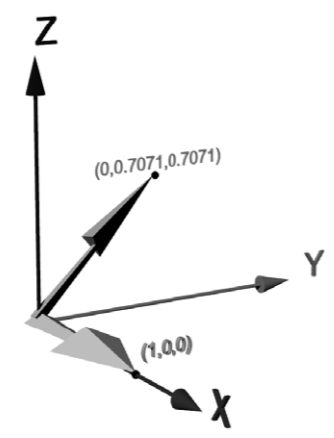
\includegraphics[width=.4\linewidth]{images/3d_start_end_rotations.png}
  \caption{Start and end rotation}
\end{subfigure}%
\begin{subfigure}{.5\textwidth}
  \centering
  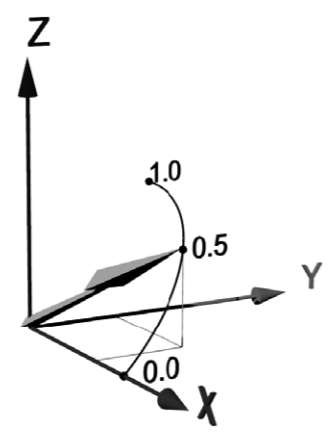
\includegraphics[width=.4\linewidth]{images/3d_interpolated_rotation.png}
  \caption{Interpolated rotation}
\end{subfigure}
\caption[Interpolation of rotations in 3D]{Interpolation of rotations in 3D \cite{ISO19141_moving_features}}
\label{fig:3d_interpolation}
\end{figure}

The interpolation process can be represented mathematically as follows. To interpolate between two rotations represented by quaternions \( q_0 \) and \( q_1 \), we first compute an angle \( \theta \) between them, and then apply the \textit{slerp} process to find the interpolated rotation. $r$ is a ratio value which depends on the instant of the resulting rotation, just as in \ref{section:interpolate}.

\begin{equation}
\begin{split}
    \cos(\theta)    & = q_0 \bullet q_1 \\
    q(r)            & = Slerp(q_0, q_1, r) \\
                    & = \frac{q_0 * \sin((1-r)*\theta) + q_1 * \sin(r*\theta)}{\sin(\theta)}
\end{split}
\end{equation}
    
\subsubsection{Interpolating 2d rotations using complex numbers}

We have shown how quaternions can be used to represent 3d rotations and to compute interpolation between 3d rotations. These techniques can thus also be used for 2d rotations, since they are a special type of 3d rotations and the interpolation between two 2d rotations also results in a 2d rotation. Nevertheless, using a quaternion rotation for 2d rotations might be overkill if 3d rotations do not need to be handled. A method has previously been described that handles only 2d rotations, but as said previously, it has to handle edge cases, because of the fact that rotation angles have to be between \( - \pi \) and \( \pi \). Another method uses complex numbers to, similarly to the previously mentioned quaternions, compute interpolation of 2d rotations in an efficient way. This is done using the exact same technique as with quaternions, but using less parameters. The equations are shown below, and the similarity with the previously defined equations for quaternions can clearly be seen.

A rotation of $\theta$ around the origin can be represented using the complex number \( q = \cos(\frac{\theta}{2}) + i*\sin(\frac{\theta}{2}) \) and a 2d point \( p = (x, y) \) can be represented using the complex number \( p = x + i*y \). Computing the interpolation between two rotations \( q_0 \) and \( q_1 \) can be done in a similar manner as quaternion interpolation

\begin{equation}
\begin{split}
\cos(\frac{\theta}{2})  &= q_0 \bullet q_1 \\
                        &= \cos(\frac{\theta_0}{2})*\cos(\frac{\theta_1}{2}) + \sin(\frac{\theta_0}{2})*\sin(\frac{\theta_1}{2}) \\
                        &= \cos(\frac{\theta_1 - \theta_0}{2}) \\
                        & \\
q(r)                &= Slerp(q_0, q_1, r) \\
                &= \frac{q_0 * \sin((1-r)*(\frac{\theta}{2})) + q_1 * \sin(r*(\frac{\theta}{2}))}{\sin((\frac{\theta}{2}))} \\
                &= \cos((1-r)*\frac{\theta_0}{2} + r*\frac{\theta_1}{2}) + i*\sin((1-r)*\frac{\theta_0}{2} + r*\frac{\theta_1}{2}) \\
\end{split}
\end{equation}

, and the same can be said for applying the rotation to an arbitrary point.

\begin{equation}
\begin{split}
    p'  &= q*p*q \\
        &= q^2*p \\
        &= (\cos(\frac{\theta}{2})^2 + \sin(\frac{\theta}{2})^2 + i*2\cos(\frac{\theta}{2})\sin(\frac{\theta}{2}))*p \\
        &= (\cos(\theta) + i*\sin(\theta))*(x + i*y) \\
        &= (x*\cos(\theta) - y*\sin(\theta)) + i*(x*\sin(\theta) + y*\cos(\theta)) \\
\end{split}
\end{equation}
%!TEX root = ../main.tex

\section{Deformable regions}
\label{section:deformable}

A last aspect of moving regions that is not handled in this thesis are the deformable moving regions. Section \ref{section:deformable_regions} describes some of the research made on this type of regions, but as explained in that section, the most common representation is not suitable for MobilityDB and has to be adapted quite a bit. This special sliced representation is used to allow for an efficient interpolation. Of course, if we are talking about regions moving in discrete time steps, this interpolation is not necessary, and the sliced representation does not offer any advantage over the MobilityDB representation. We can thus split the set of deformable moving regions in two.

A deformable region subject to continuous transformations is the most difficult type to handle, but is also the type most present in real-life: boundaries of forests, ponds, oil leaks in the ocean, clouds, etc. However, as said previously, the current solutions for this type of region is quite far from the MobilityDB implementation, so it will not be discussed further. Regions changing in discrete time steps, however, can be implemented without too much trouble in MobilityDB, and this is discussed below.

Note that, contrary to all previous section, these ideas have not been tested in practice, so this is only a discussion and not a presentation of results.

\subsubsection{Discrete movement}

The main issue when handling deformable regions is that the value of the region between two defined instants is hard to interpolate. For regions that move in discrete time steps, this is not the case anymore, since this value is equal to the one stored in the last instant. Since interpolation is not an issue anymore, we do not have to adapt the representation and this type of moving regions can thus be represented easily using the internal MobilityDB representation. 

\[
    '\{[\mathcal{R}_0^0@t_0^0,\ \mathcal{R}_1^0@t_1^0,\ ...],\ [\mathcal{R}_0^1@t_0^1,\ \mathcal{R}_1^1@t_1^1,\ ...],\ ...\}'
\]

, where all region values $\mathcal{R}_i^i$ are different from each other, because we handle deformable regions.

This representation would be totally acceptable and all the needed functions could be implemented to handle this new type. The only true issue that I can see with this representation is that the memory size might become large when handling large sequences/set. One possible solution would be to store a difference between the current region and the previous one if this is smaller than the current region, but depending on the changes that the region undergoes, this might not be beneficial.

One good example of a use case for this type of regions is a \textit{cadastre}, which records the ownership of land parcels in countries. Cadastral updates are by nature discrete, and the different parcels in a cadastre could thus be represented like shown above.

Implementing of this new region type, and testing if and how it could be used for real-world applications such as cadastres is left as future work.

 
\chapter{Conclusion}
\lipsum[2-4]

\appendix

\chapter{Complete List of Transformation Functions}
%!TEX root = ../main.tex
\label{appendix:complete_funct_tables}

\begin{table}[htbp]
\begin{subtable}{1\textwidth}
\centering
    \begin{tabularx}{\textwidth}{|l|X|}
        \hline
        \textbf{Function}   & \textbf{Signature} \\ 
        \hline
        \lstinline+duration+            & \lstinline+tgeometry+ $\rightarrow$ \lstinline+text+\\
        \hline
        \lstinline+interpolation+       & \lstinline+tgeometry+ $\rightarrow$ \lstinline+text+\\
        \hline
        \lstinline+memSize+             & \lstinline+tgeometry+ $\rightarrow$ \lstinline+integer+ \\
        \hline
        \lstinline+getValue+            & \lstinline+tgeometry(Instant)+ $\rightarrow$ \lstinline+geometry(Polygon)+ \\
        \hline
        \lstinline+startValue+          & \lstinline+tgeometry+ $\rightarrow$ \lstinline+geometry(Polygon)+ \\
        \hline
        \lstinline+endValue+            & \lstinline+tgeometry+ $\rightarrow$ \lstinline+geometry(Polygon)+ \\
        \hline
        \lstinline+getTimestamp+        & \lstinline+tgeometry(Instant)+ $\rightarrow$ \lstinline+timestamptz+ \\
        \hline
        \lstinline+getTime+             & \lstinline+tgeometry+ $\rightarrow$ \lstinline+periodset+ \\
        \hline
        \lstinline+timespan+            & \lstinline+tgeometry+ $\rightarrow$ \lstinline+interval+ \\
        \hline
        \lstinline+shift+               & \lstinline+tgeometry+ $\rightarrow$ \lstinline+tgeometry+ \\
        \hline
        \lstinline+numInstants+         & \lstinline+tgeometry+ $\rightarrow$ \lstinline+integer+ \\
        \hline
        \lstinline+startInstant+        & \lstinline+tgeometry+ $\rightarrow$ \lstinline+tgeometry(Instant)+ \\
        \hline
        \lstinline+endInstant+          & \lstinline+tgeometry+ $\rightarrow$ \lstinline+tgeometry(Instant)+ \\
        \hline
        \lstinline+instantN+            & \lstinline+tgeometry+ $\times$ \lstinline+integer+ $\rightarrow$ \lstinline+tgeometry(Instant)+ \\
        \hline
        \lstinline+instants+            & \lstinline+tgeometry+ $\rightarrow$ \lstinline+array tgeometry(Instant)+ \\
        \hline
        \lstinline+numTimestamps+       & \lstinline+tgeometry+ $\rightarrow$ \lstinline+integer+ \\
        \hline
        \lstinline+startTimestamp+      & \lstinline+tgeometry+ $\rightarrow$ \lstinline+timestamptz+ \\
        \hline
        \lstinline+endTimestamp+        & \lstinline+tgeometry+ $\rightarrow$ \lstinline+timestamptz+ \\
        \hline
        \lstinline+timestampN+          & \lstinline+tgeometry+ $\times$ \lstinline+integer+ $\rightarrow$ \lstinline+timestamptz+ \\
        \hline
        \lstinline+timestamps+          & \lstinline+tgeometry+ $\rightarrow$ \lstinline+array timestamptz+ \\
        \hline
        \end{tabularx}
\end{subtable}
\caption{Transformation functions (complete)}
\label{table:transformation_funcs_complete}
\end{table}

\clearpage

\begin{table}[htbp]
\ContinuedFloat
\begin{subtable}{1\textwidth}
\centering
    \begin{tabularx}{\textwidth}{|l|X|}
    \hline
    \textbf{Function}   & \textbf{Signature} \\ 
    \hline
    \lstinline+numSequences+        & \lstinline+tgeometry+ $\rightarrow$ \lstinline+integer+ \\
    \hline
    \lstinline+startSequence+       & \lstinline+tgeometry+ $\rightarrow$ \lstinline+tgeometry(Sequence)+ \\
    \hline
    \lstinline+endSequence+         & \lstinline+tgeometry+ $\rightarrow$ \lstinline+tgeometry(Sequence)+ \\
    \hline
    \lstinline+SequenceN+           & \lstinline+geometry+ $\times$ \lstinline+integer+ $\rightarrow$ \lstinline+tgeometry(Sequence)+ \\
    \hline
    \lstinline+Sequences+           & \lstinline+tgeometry+ $\rightarrow$ \lstinline+array tgeometry(Sequence)+ \\
    \hline
    \end{tabularx}
\end{subtable}
\caption{Transformation functions (complete), continued}
\end{table}

\chapter{Conversions Between 3D Rotation Representations}
%!TEX root = ../main.tex
\label{appendix:rot_repr_conversions}

\nocite{*}
\printbibliography
\note{Check copyright for ISO reference!}

\end{document}